%% thesis.tex 2014/04/11
%
% Based on sample files of unknown authorship.
%
% The Current Maintainer of this work is Paul Vojta.

\documentclass[masters]{ucbthesis}
\usepackage{biblatex}
\usepackage{rotating} % provides sidewaystable and sidewaysfigure
\usepackage{float}
\usepackage{amsmath}
\usepackage[inkscapeformat=png]{svg}

% To compile this file, run "latex thesis", then "biber thesis"
% (or "bibtex thesis", if the output from latex asks for that instead),
% and then "latex thesis" (without the quotes in each case).

% Double spacing, if you want it.  Do not use for the final copy.
% \def\dsp{\def\baselinestretch{2.0}\large\normalsize}
% \dsp

% If the Grad. Division insists that the first paragraph of a section
% be indented (like the others), then include this line:
% \usepackage{indentfirst}

\addtolength{\abovecaptionskip}{\baselineskip}

\newtheorem{theorem}{Jibberish}

\bibliography{references}

\hyphenation{mar-gin-al-ia}
\hyphenation{bra-va-do}

\begin{document}

% Declarations for Front Matter

\title{Implementation of an Open-Source Generator for LPDDR4X Memory Controller}
\author{Reza Sajadiany}
\degreesemester{Spring}
\degreeyear{2023}
\degree{Master of Science}
\chair{Professor Borivoje Nikolic}
\othermembers{Professor Sophia Shao, Second Reader}
% For a co-chair who is subordinate to the \chair listed above
% \cochair{Professor Benedict Francis Pope}
% For two co-chairs of equal standing (do not use \chair with this one)
% \cochairs{Professor Richard Francis Sony}{Professor Benedict Francis Pope}
\numberofmembers{3}
% Previous degrees are no longer to be listed on the title page.
% \prevdegrees{B.A. (University of Northern South Dakota at Hoople) 1978 \\
%   M.S. (Ed's School of Quantum Mechanics and Muffler Repair) 1989}
\field{Electrical Engineering and Computer Science}
% Designated Emphasis -- this is optional, and rare
% \emphasis{Colloidal Telemetry}
% This is optional, and rare
% \jointinstitution{University of Western Maryland}
% This is optional (default is Berkeley)
% \campus{Berkeley}

% For a masters thesis, replace the above \documentclass line with
% \documentclass[masters]{ucbthesis}
% This affects the title and approval pages, which by default calls this
% document a "dissertation", not a "thesis".

\maketitle
% Delete (or comment out) the \approvalpage line for the final version.
\approvalpage
\copyrightpage

% (This file is included by thesis.tex; you do not latex it by itself.)

\begin{abstract}

% The text of the abstract goes here.  If you need to use a \section
% command you will need to use \section*, \subsection*, etc. so that
% you don't get any numbering.  You probably won't be using any of
% these commands in the abstract anyway.

As the software requirements for hardware implementations become more complex, the need for agile development of a full system becomes more apparent. The design of complex hardware systems requires engineering efforts at different levels of abstraction layers. This design process becomes more efficient when the units that make up a system are separated by defined interfaces and communicate over a fixed protocol. A full system in the context of a system-on-chip must adhere to protocols defined at the architectural level. Once such protocol is defined for memory devices. Today's workloads are often data-driven and need to access larger working sets of memory; however, the on-die memory system is limited by area and the power envelope of the target design. An off-chip volatile memory provides high-density memory implemented in less complex transistor nodes and provides the benefit of a large backing memory for the whole system. 

In addition, the most significant delays in modern systems are due to cache misses and cache refills from the DRAM. A typical delay estimate for such events is believed to be on the order of hundreds of cycles of the CPU clock. A memory controller is a crucial unit in the system that contributes to cache refill delays and the efficiency and bandwidth of the memory hierarchy. 

LPDDR4X represents a generation of memory devices defined by the JEDEC organization that implement the defined set of functionalities specified by the JEDEC standard for memory devices. This common standard unifies the protocol the memory controller designer needs to implement for a compatible DRAM device to function properly. In this thesis, I will describe my contribution to the implementation of a compatible memory controller design. This thesis focuses on an overview of the LPDDR4X and DRAM, design specifications and requirements, the architecture, and the micro-architecture of our LPDDR4X implementation. This implementation is included in UC Berkeley's Chipyard SoC generator and has been done in the Chisel hardware description language.
\end{abstract}


\begin{frontmatter}

\begin{dedication}
\null\vfil
\begin{center}
I dedicate this work to my parents who sacrificed many to give me the opportunity of a lifetime. 
\end{center}
\vfil\null
\end{dedication}

% You can delete the \clearpage lines if you don't want these to start on
% separate pages.

\tableofcontents
\clearpage
\listoffigures
\clearpage
\listoftables

\begin{acknowledgements}

This project was conducted under the supervision and support of Professor Borivoje Nikolic and Sophia Shao at the UC Berkeley Slice lab and Berkeley Wireless Research Center.

I would like to acknowledge graduate student researcher Ken Ho who I worked with from the beginning phase of the project. The LPDDR4 project is a shared effort and work by Ken Ho and myself. The project will be maintained and further investigation in the area will continue by Ken Ho and other graduate and undergraduate students in the future. 

I acknowledge the help and support of Jennifer Zhou for keeping me on track during the course of my Master's degree.


I would like to acknowledge graduate student researchers at UC Berkeley's Slice lab and Berkeley Wireless Research Center namely Jerry Zhao, Vighnesh Iyer, Daniel Grubb, Harrison Liew, Abraham Gonzales, and Sagar Karandikar.

In this project, we referenced work done by Chipyard developers. I would like to thank the Chipyard development team and the Hammer development team.

Finally, I would like to acknowledge Apple for its generous assistance to my Master's degree by providing me with guidance, internship, and scholarship. 
\end{acknowledgements}

\end{frontmatter}

\pagestyle{headings}

% (Optional) \part{First Part}

\chapter{Overview of LPDDR4X}

\section{DRAM and LPDDR4X}
DRAM, or dynamic random access memory, is a type of volatile memory that is widely used in digital electronic systems. Volatile memory is a type of memory that loses its stored data when the power is turned off. DRAM operates by storing each data bit in a separate capacitor within a memory cell. The charge stored in each capacitor represents the binary value of the bit.

To maintain the data stored in the memory cells, a periodic refresh operation must be performed, hence the name “dynamic” memory. The refresh operation essentially rewrites the data in the memory cells to prevent the loss of data as the charge in the capacitor of a memory cell leaks out of the cell.

In DRAM, data is accessed randomly, as any memory location can be accessed directly without having to access the memory in a specific order, hence the term “random access” memory. This random access capability of DRAM provides faster access to data compared to other types of memory, such as magnetic disk drives.

DRAM technology is based on a capacitor-transistor (C-T) cell, which consists of an access transistor and a trench capacitor \cite{BORA}. The transistor allows current to go through and control the flow of charge to and from the capacitor. During a read operation, the charge stored in the capacitor is sensed and converted into a digital voltage signal, which represents the binary value of the data. During a write operation, the voltage signal is converted into a charge and stored in the capacitor.
DDR stands for double data rate and is an indication of the device sampling data and sending data twice per clock cycle. This is done by sampling the data on crossing points of a differential clock pair. Figure \ref{fig:dram-io} depicts the signals for double data sampling. 
A memory device is organized to maximize memory bandwidth and minimize the latency of operations. The organization of a DRAM module allows the designer of the memory controller to take advantage of parallel channels and structures to increase the data bandwidth. 

The device specification of each generation such as LPDDR4 (Low-power Double Data Rate) is defined by the JEDEC organization \cite{jedec}. Table \ref{tab:standards} shows multiple generations of the DDR standards up to DDR4 and the corresponding clock rate and transfer bandwidth \cite{patterson}. Amdahl's law suggests that the capacity of DRAM devices needs to grow linearly with the processor speeds; however, the performance and capacity of DRAM devices are growing at a much slower rate \cite{patterson}. 
\begin{table}[]
    \centering
    \begin{tabular}{c|c|c|c|c}
         Standard & Release Year & Capacity & I/O Clock Rate & MiB/s/DIMM \\
         \hline
         DDR1 & 2000 & 256 MB & 133 & 2128 \\
         DDR2 & 2004 & 1 GB & 266 & 4264 \\
         DDR3 & 2010 & 4 GB & 533 & 8528 \\
         DDR4 & 2016 & 8 GB & 1333 & 21300\\
    \end{tabular}
    \caption{DDR standards \cite{patterson}.}
    \label{tab:standards}
\end{table}
Functional description, detailed device operations, bus operations, cycle-accurate timings, and nominal conditions of operations are described in the 
specification for each generation. 
\section{DRAM Organization}

\begin{figure}[h]
    \centering
    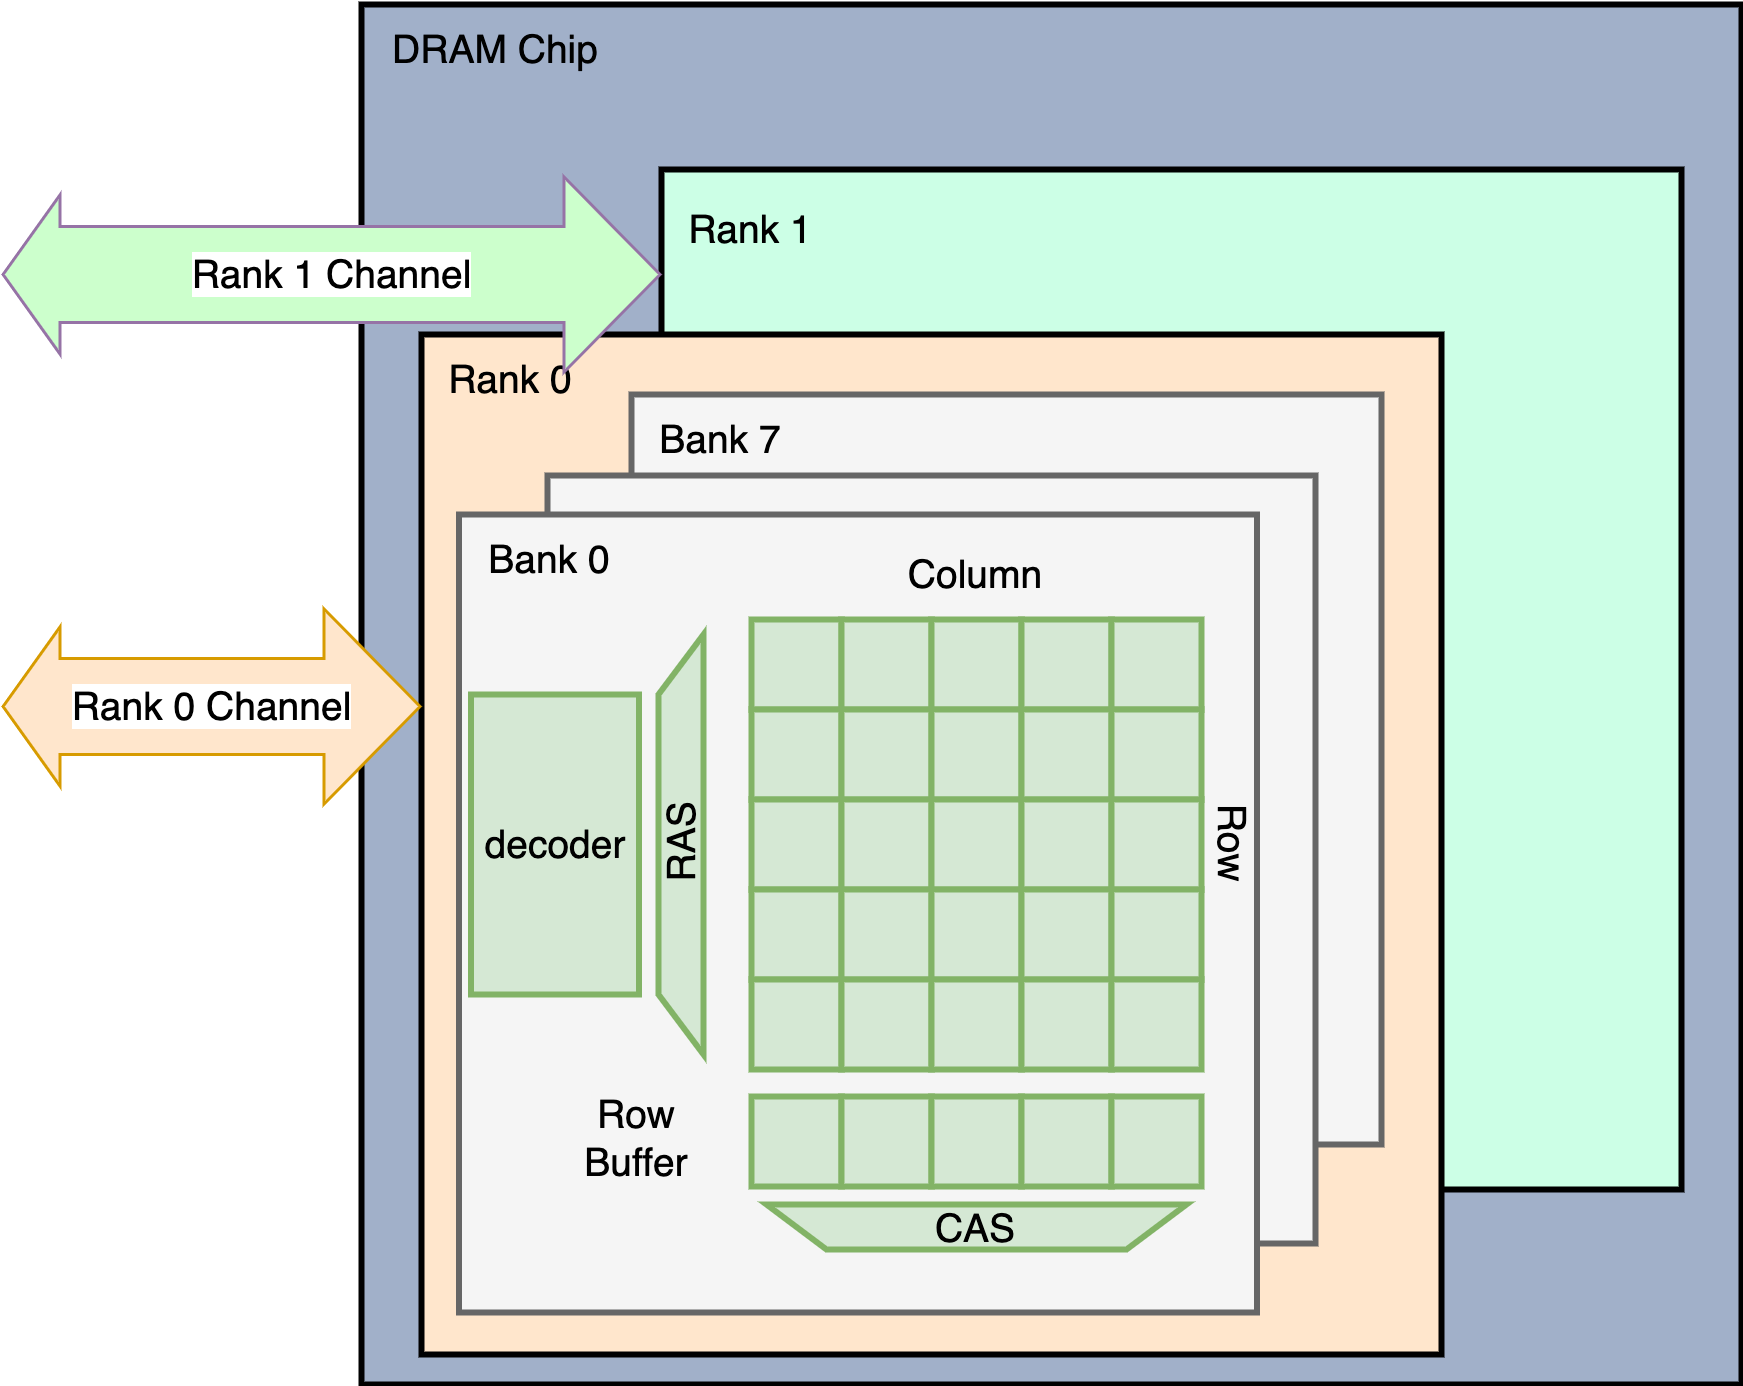
\includegraphics[scale=.14]{images/rank-bank.png}
    \caption{DRAM device organization.}
    \label{fig:rank-bank}
\end{figure}

DRAM devices are optimized to increase the bandwidth of the memory channels. The metric for such optimization is the activity of the DQ lanes between the DRAM and the controller. DQ is a bi-directional bus between the device and the memory controller. The organization and internals of the DRAM device dictate the complexity and responsibilities of a DRAM controller. As depicted in Figure \ref{fig:rank-bank}, a typical LPDDR4X device is organized into two physically separated ranks. Each rank of the device can be configured and connected to a separate channel. These two ranks can be active simultaneously and operate independently of each other. Each rank is organized into 8 banks of memory. The states of these banks impact the overall state of the memory device. Each bank is a two-dimensional memory array with column and row addresses. The memory array is structured as capacitor-based bit-cells with an access transistor for accessing the data stored in the capacitor. A row can store a large set of bytes and can extend to multiple system cache lines. A subset of the row is selected by multiplexers based on the column address. To perform a read transaction: the corresponding bank within the rank must be selected based on the address; the row for which the address maps to is selected, and the columns corresponding to the requested address are selected. Each operation must perform a sequence of specified commands to be issued to a bank for the purpose of reliably reading the data from the memory. The example read operation above would require activation of the row or row access (RAS), followed by a column access command (CAS), and finally by a pre-charge command (PRE). The timing and latencies between each step are specified by the JEDEC specification and the memory controller is responsible for obeying them. Overall, the memory controller is responsible for issuing the right sequence of commands at the right time to the device. Internally the memory controller must keep track of the state of the device at each cycle, allow the legal commands to be issued at any point, and force the right ordering of the commands. The timing requirements introduce the opportunity to optimize the memory controller to take full advantage of the possible bandwidth by allowing the architect to re-order requests, delay a pre-charge, or delay a refresh.
\section{DRAM Interface}
\begin{figure}
    \centering
    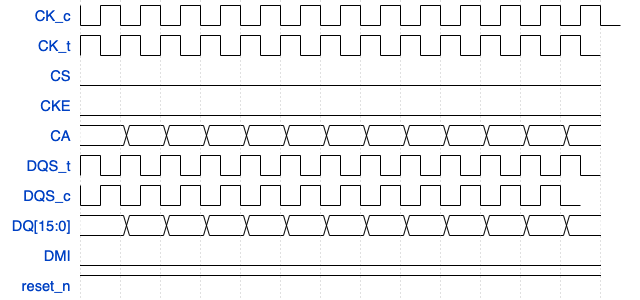
\includegraphics[scale=0.5]{images/signals.png}
    \caption{Waveform of device signals.}
    \label{fig:dram-io}
\end{figure}
\begin{figure}
    \centering
    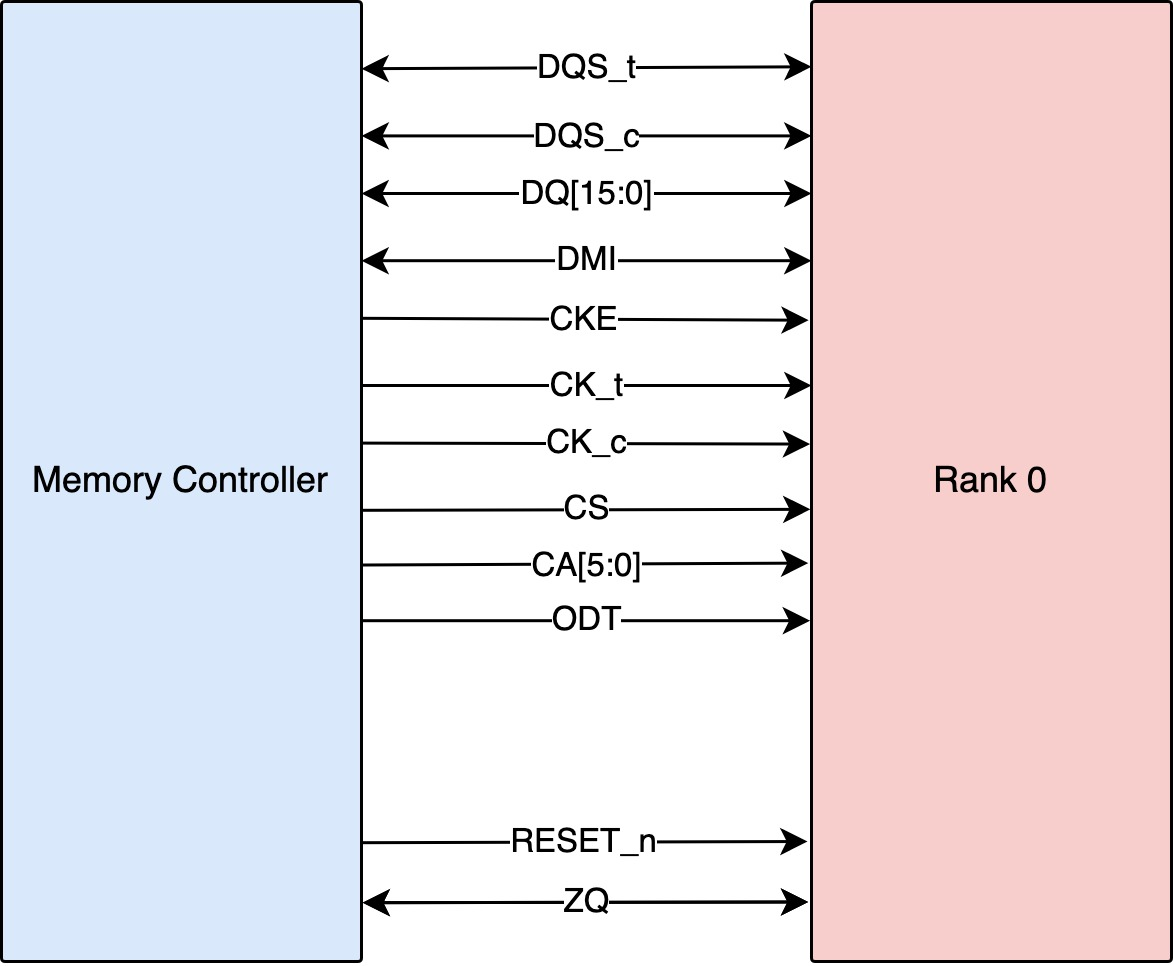
\includegraphics[scale=0.2]{images/signal-int.jpg}
    \caption{Signal interface for x16.}
    \label{fig:sig-int}
\end{figure}

The JEDEC specification determines the standard signals to be driven by the DDR controller and the DRAM device. An example of a signal waveform is shown in Figure \ref{fig:dram-io}. A description of each signal is shown based on the JEDEC specification in Table \ref{tab:signal-def}. Each LPDDR4X DRAM device is divided into two ranks which are connected in parallel to a dedicated channel. Signals such as CK\_t and CK\_c are shared among the two channels; however, the DQ bus, the CA bus, and the corresponding differential DQS clocks are separate between the two channels. 
\begin{table}[]
    \centering
    \begin{tabular}{c|c|c}
         Symbol & Type &  Description\\
         \hline
         CK\_t | CK\_c & Input & Clock: CK\_t and CK\_c are differential clock inputs\\
         CKE & Input & Clock Enable: Active high signal\\
         CS & Input & Chip Select \\
         CA[5:0] & Input & Command and Address Inputs\\
         ODT & Input & On-Die-Termination control\\
         DQ[15:0] & I/O & Bi-directional data input and output\\
         DQS\_t | DQS\_c & I/O & Data Strobe, Bi-directional differential clock signal\\
         DMI & I/O & Data Mask Inversion \\
         ZQ & Reference & Calibration Reference \\
         RESET\_n & Input & Active low reset signal
    \end{tabular}
    \caption{Signal Description for x16.}
    \label{tab:signal-def}
\end{table}
\newpage
\section{Prior Work}
Research on memory controllers in universities and among academics has a very short background. To our knowledge, many other research institutions either do not work in this area, or purchase vendor IP to integrate in their design. In the open-source community, LiteDRAM by EnjoyDigital \cite{enjoydigital} is an implementation of a DDR4 controller that can be mapped to FPGA systems. However, for the purposes of enabling more research work to be done in this area, an open-source controller is required.
\section{Project Goals}
The target for this project was to design an open-source LPDDR4X controller to be used as an IP in chip designs, and to be used to study a complete SoC. Interesting work such as studying DRAM targetted attacks, system-level analysis, and reordering of transactions will be possible using such IPs. The project will result in a generator in Chipyard \cite{chipyard}. Chipyard will provide an SoC designer with simple-to-use configuration-based knobs to include IPs such as an LPDDR4X controller in a design.
\chapter{Memory Controller Architecture}
\label{chap:arch}
\section{Memory Hierarchy Organization}
\begin{figure}
    \centering
    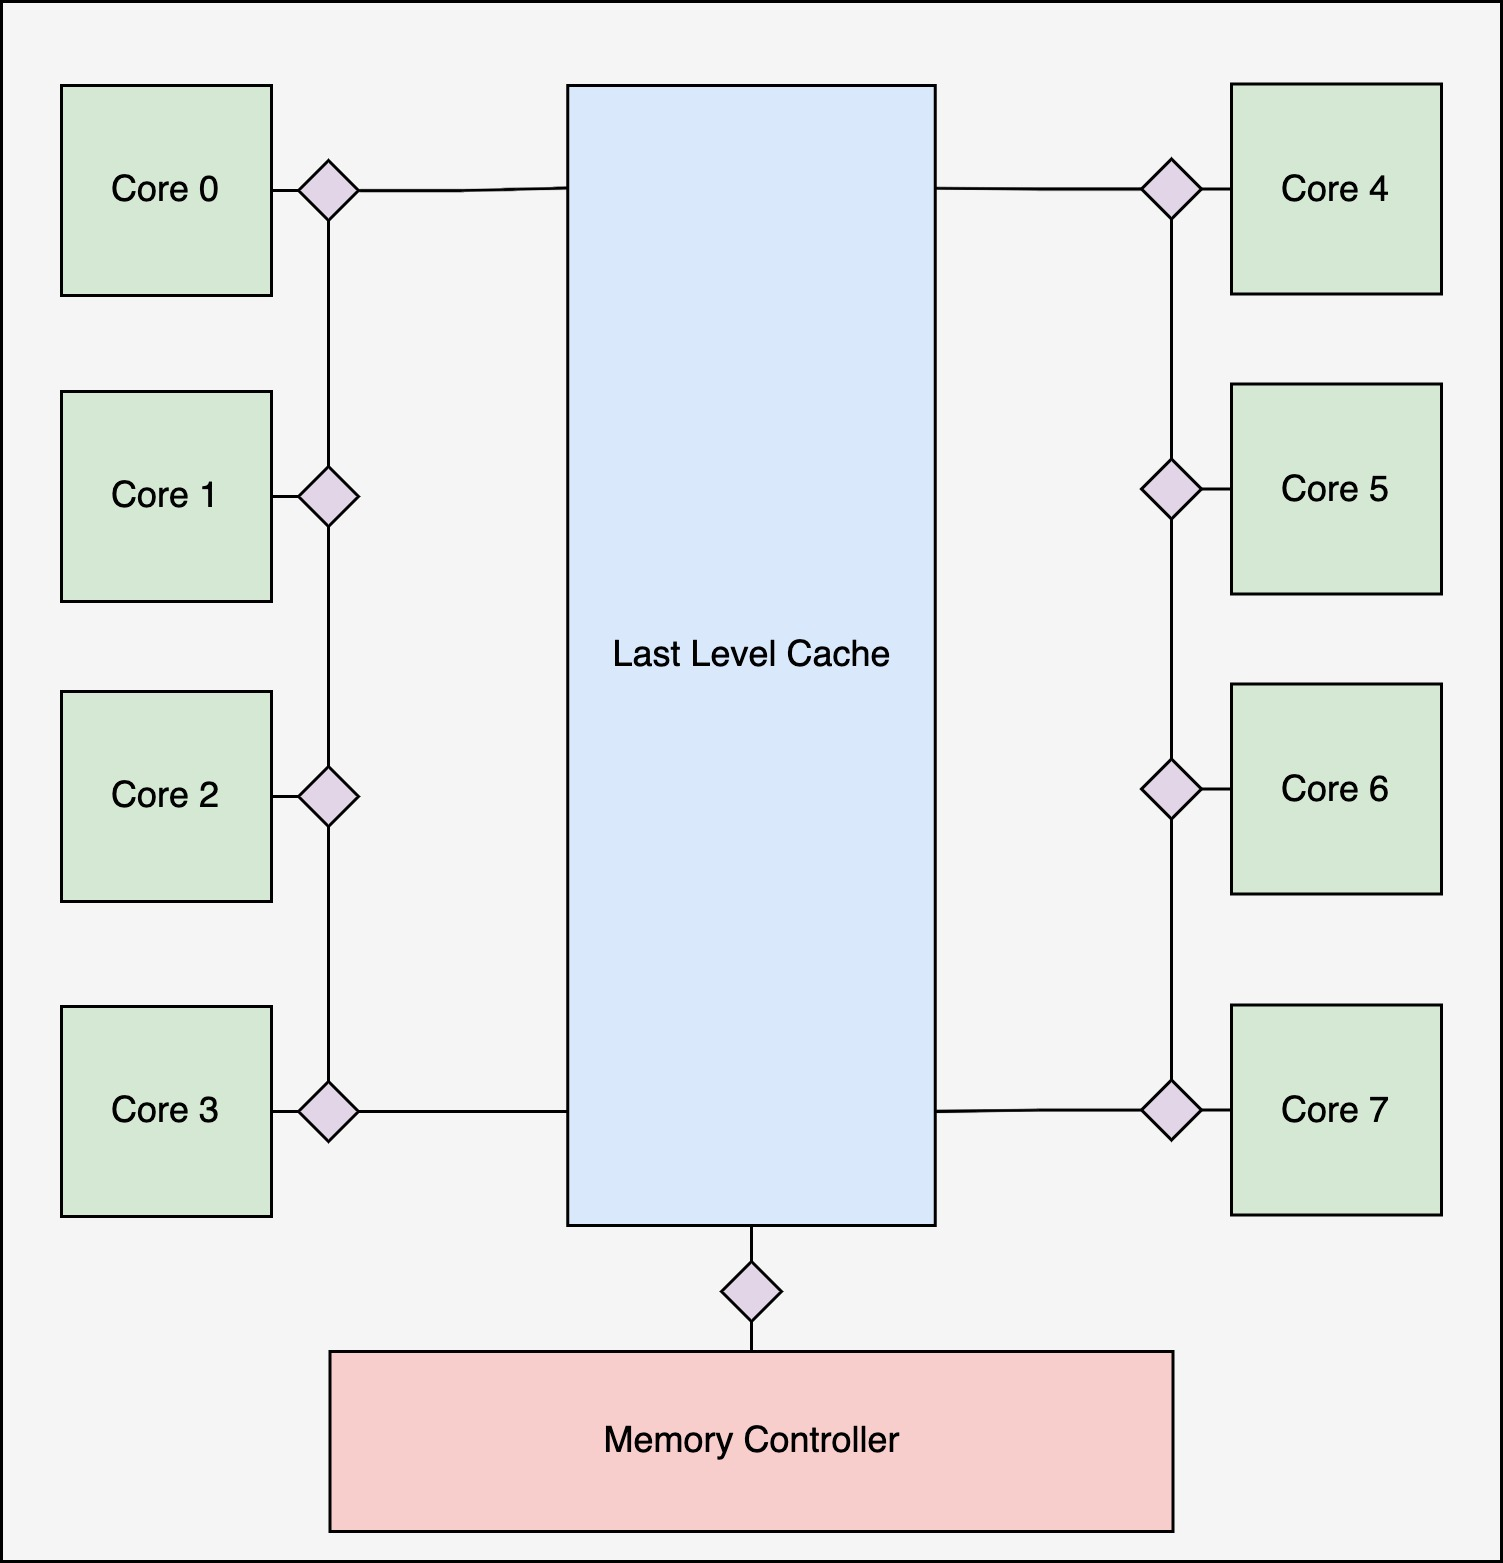
\includegraphics[scale=0.15]{images/soc-2.jpg}
    \caption{A modern SoC with 8 cores and last-level cache.}
    \label{fig:soc-2}
\end{figure}
An SoC design is organized as nodes of processing elements such as CPUs or accelerators, on-die memory systems such as L2 caches or Last Level Cache (LLC), and memory and IO controllers. A DRAM controller in such systems provides backing memory to the whole system and allows for larger programs and data to be processed on the die by caching the working subset of memory. Figure \ref{fig:soc} shows a modern memory hierarchy and system. CPU clusters are shown to have private level one and two caches; a system-level cache provides a larger pool of memory and is backed by DRAM. This project pieces together the memory controller and the physical layer to be used for the future implementation of such systems. In Figure \ref{fig:soc-2} and \ref{fig:soc}, a modern SoC is depicted with eight processing elements, a shared LLC, and a memory controller. The purple diamonds are routers as part of the SoC interconnects. One such node is connected to the memory controller. 

\begin{figure}[b]
  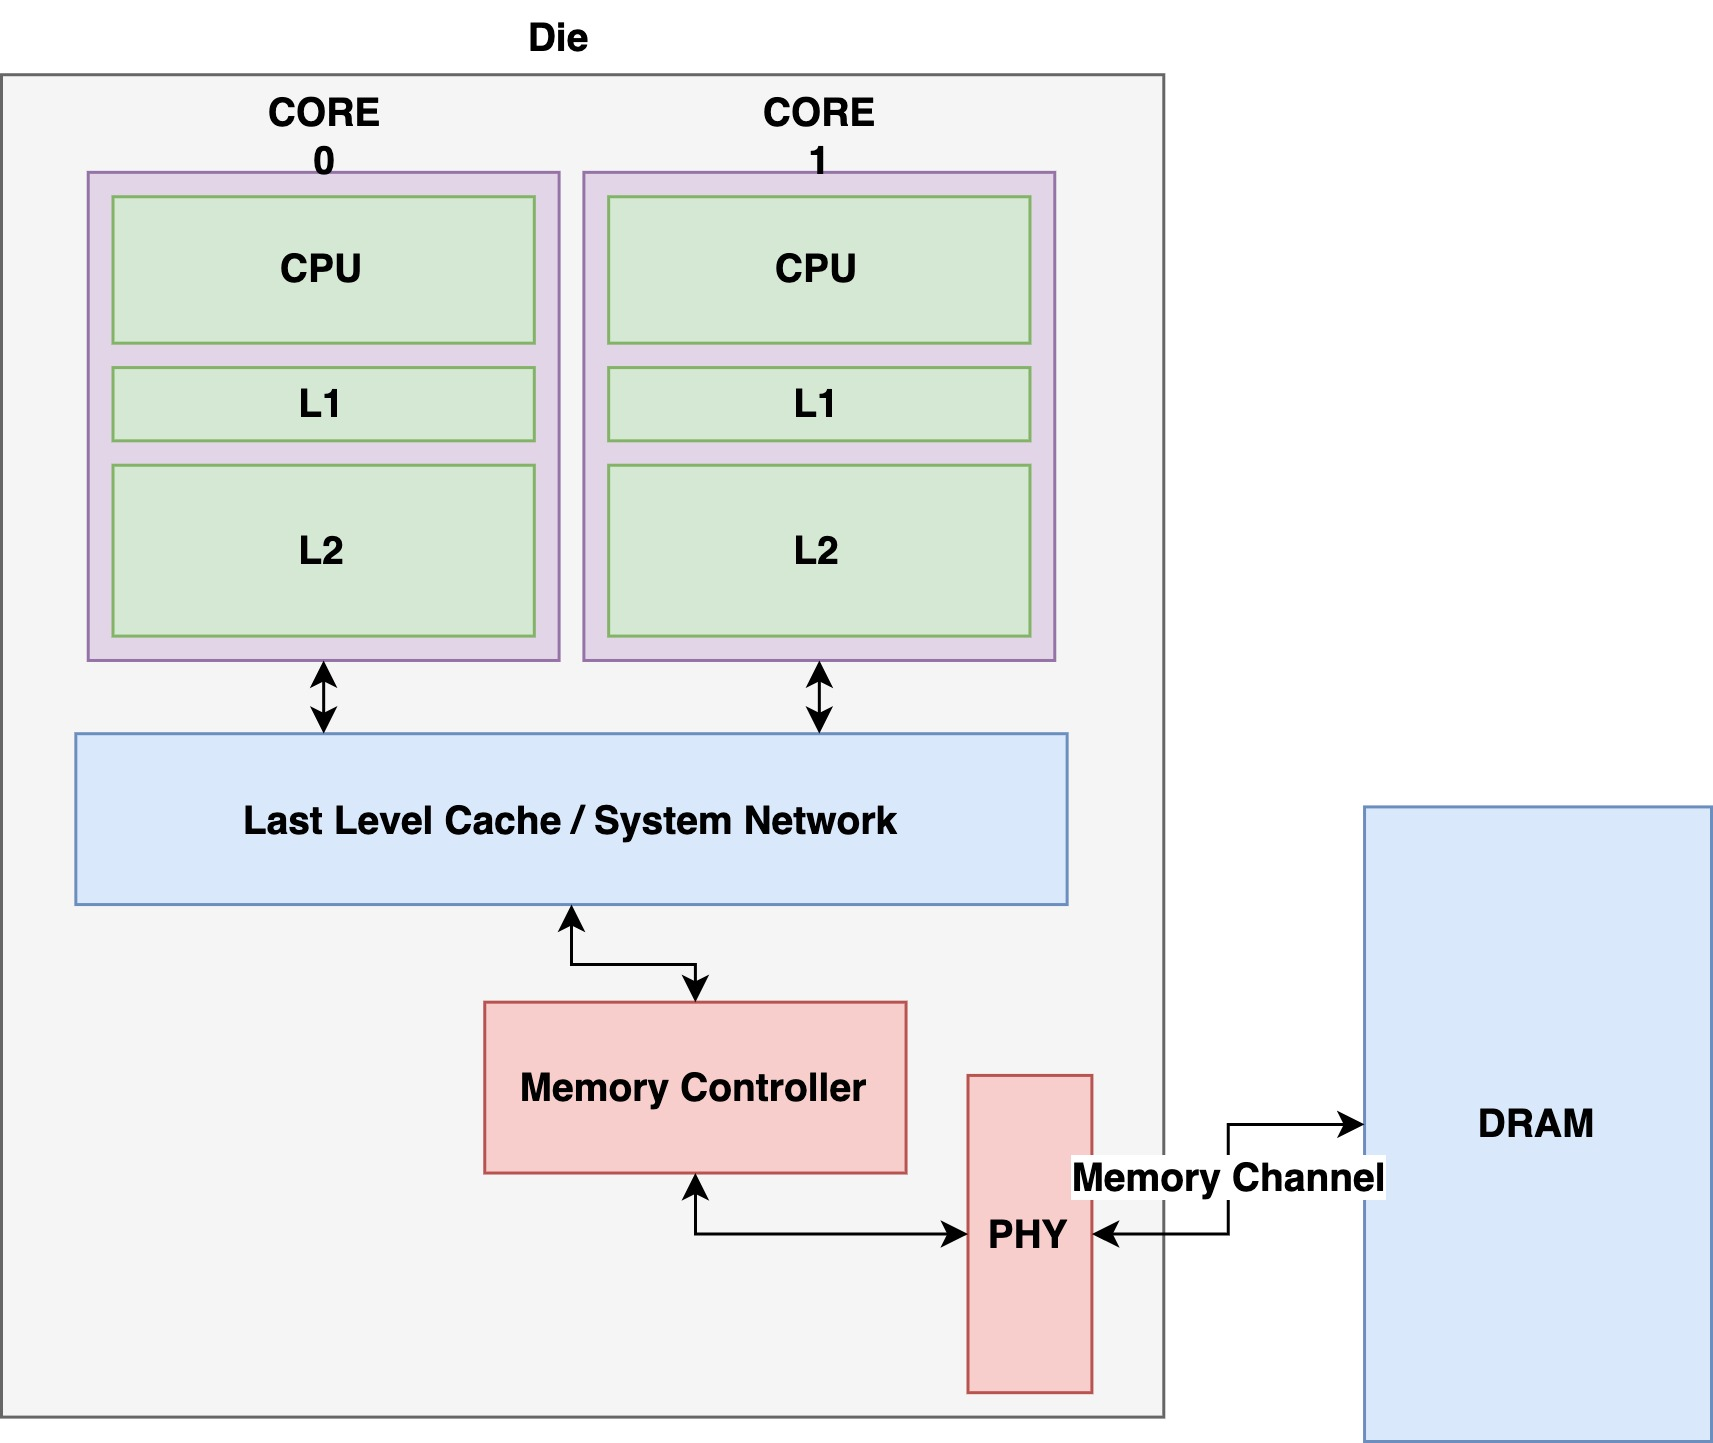
\includegraphics[scale=.15]{images/soc.jpg}
  \caption{Logical view of the memory hierarchy.}
  \label{fig:soc}
\end{figure}


As SoC architects, we should be able to perform early-stage modeling of systems by taking advantage of software modeling. A DRAM controller software model gives early estimates of system-level performance and bottlenecks. Rapid cycles of RTL software modeling is the approach taken to design complex systems. This implementation of the LPDDR4 memory controller allows for such models to be deployed and connected to the LPDDR4 model as well for more realistic performance analysis.
\section{TileLink Front-end}


\begin{figure}
    \centering
    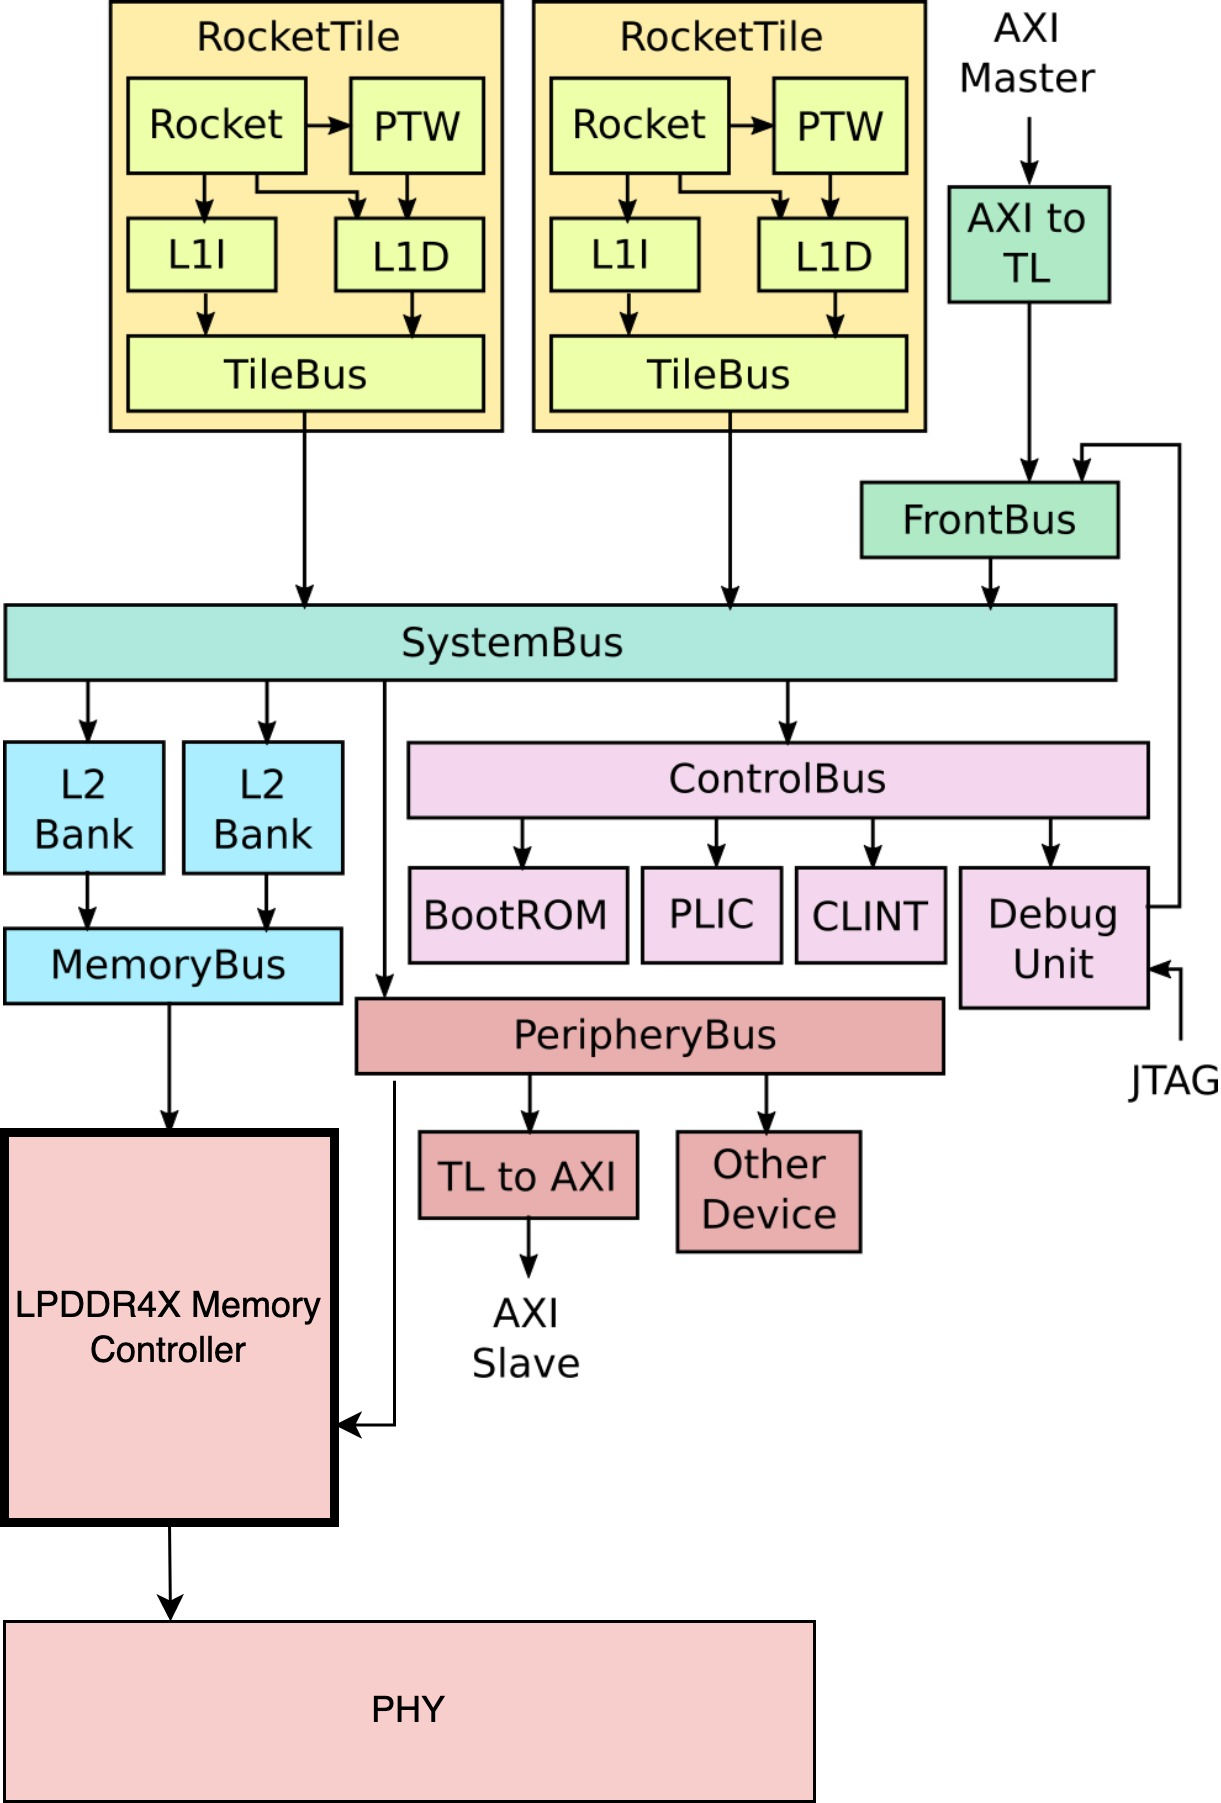
\includegraphics[scale=0.2]{images/bus.jpg}
    \caption{Bus hierarchy with LPDDR4X controller.}
    \label{fig:bus}
\end{figure}

TileLink is a logical transmission protocol to communicate messages, data, and cache coherency packets to other agents in the system \cite{tilelink}. During the design elaboration, TileLink agents of the system perform an agreement to ensure that the system is connected logically, and is free of problems such as deadlocks. For that, Chipyard \cite{chipyard}, an SoC generator, uses diplomacy to conduct the diplomatic agreement between all the agents in the system. This agreement happens at compilation time such that the system is guaranteed to have no cycles. The Diplomacy directed acyclic graph or DAG generates an SoC configuration to be elaborated. TileLink differentiates the nodes in the system based on which node is a source and which node is a sink node. A manager node (sink node) is a node that takes in requests and provides responses. TileLink protocol requires the implementation of channels A and D for a manager agent. On the other hand, a client node is a node that issues requests to other agents in the system. A CPU core in the system has a client node attached to its interface to the network. On the other hand, the memory controller has a manager node to receive requests and respond to them. To implement an interface for an SoC, the DDR controller instantiates a manager node and connects it to the memory bus of the system. In the context of the memory controller, the manager node receives only put and get requests over channel A. A put request is a data transfer from a client node to the manager node such as a write-back to a lower-level cache. Similarly, a get request is a request for data from an address. The manager node is able to respond to the requests over channel D. In addition to the manager node, the DDR controller requires a register node for the configuration of the internal registers. Figure \ref{fig:bus} shows the bus hierarchy in Chipyard and the connection of the LPDDR4X controller to the memory bus and periphery bus. Figure \ref{fig:reg-node} shows the register node is connected to the periphery bus or the PBUS of the system. The register node is needed for providing the controller with a register space that software can write to. The registers are used to control the timing parameters described in the next chapter, control and status registers, and mode registers of the DRAM device.  Each manager node can use the A and D channels of TileLink. Requests are delivered to the manager node via the A channel, and responses are delivered to the network via the D channel. Figure \ref{fig:tli}  shows a block diagram of the manager node in more detail. The logic within the manager node needs to provide two decoupled (ready-valid) interfaces to each side of the module.

\begin{figure}
    \centering
    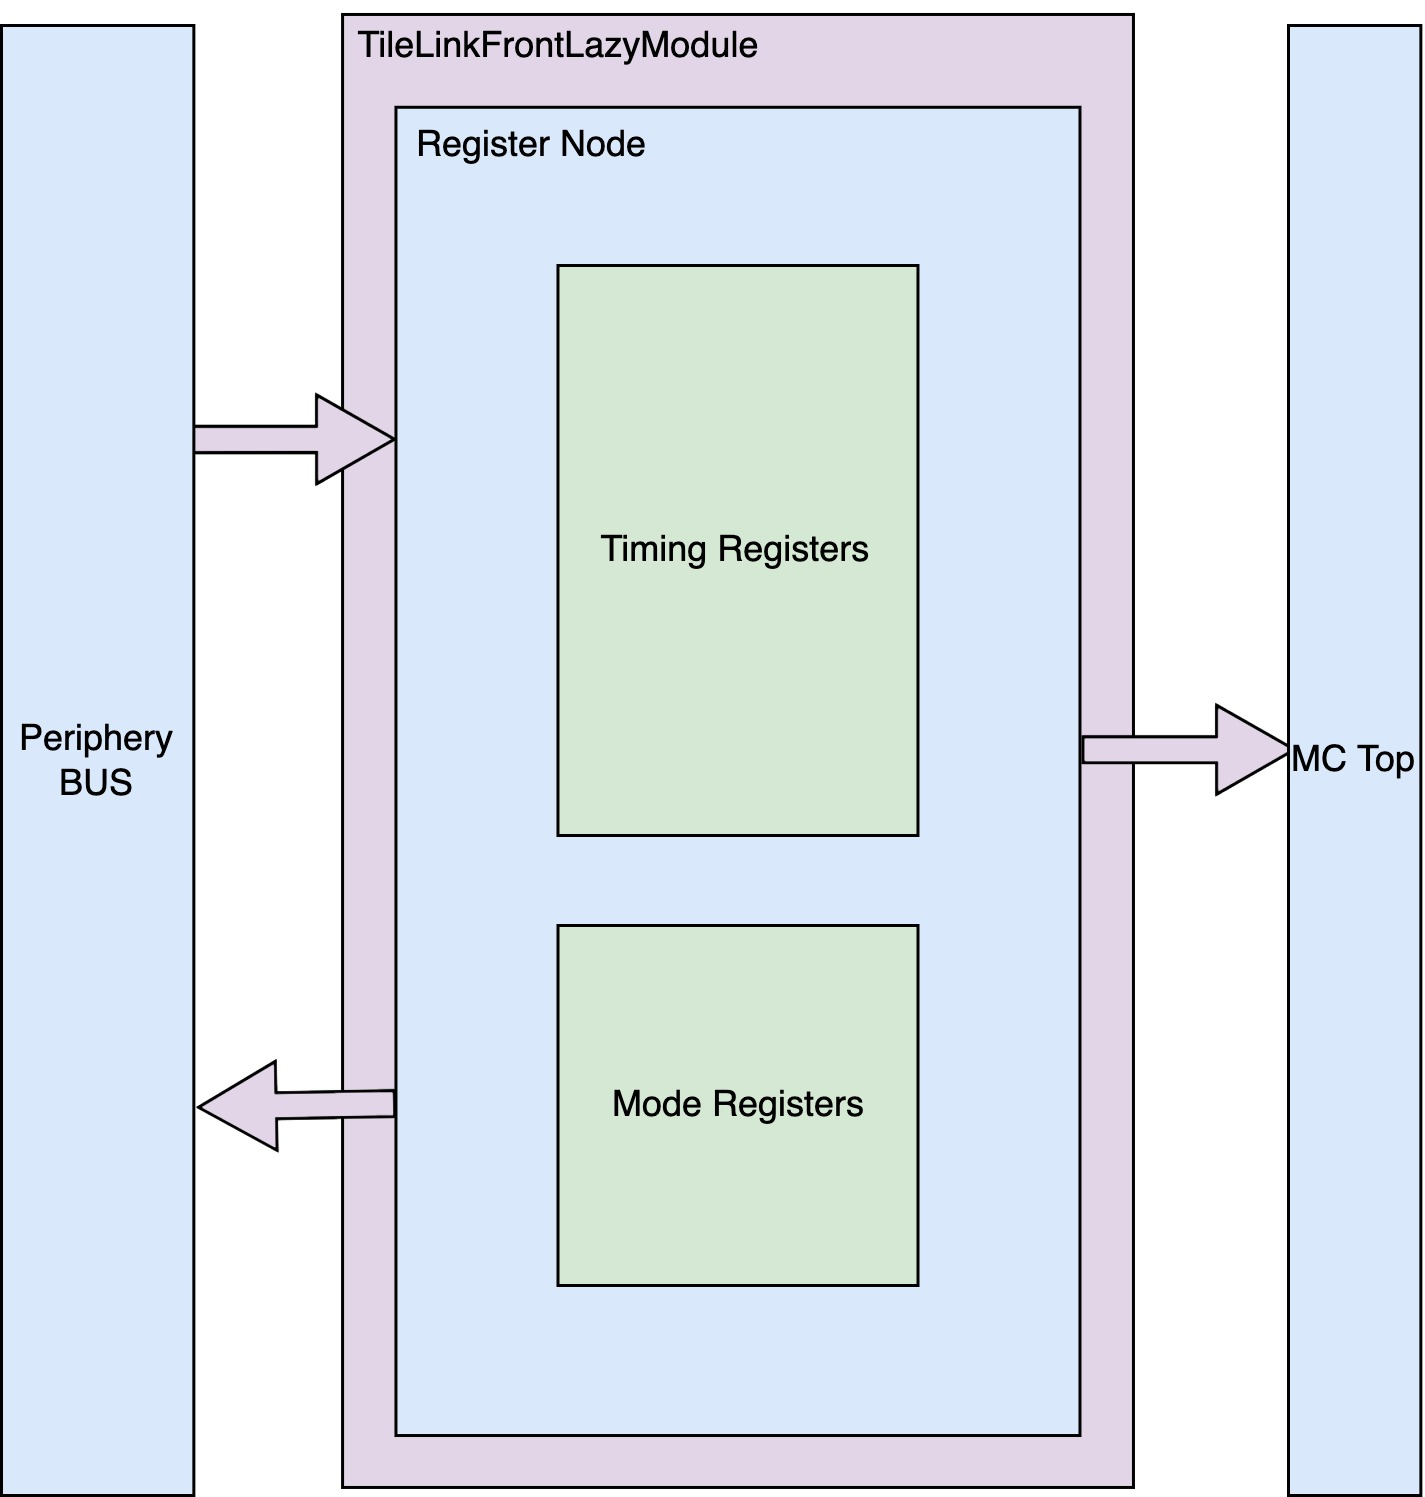
\includegraphics[scale=0.1]{images/reg-node.jpg}
    \caption{Register node.}
    \label{fig:reg-node}
\end{figure}
\begin{figure}
    \centering
    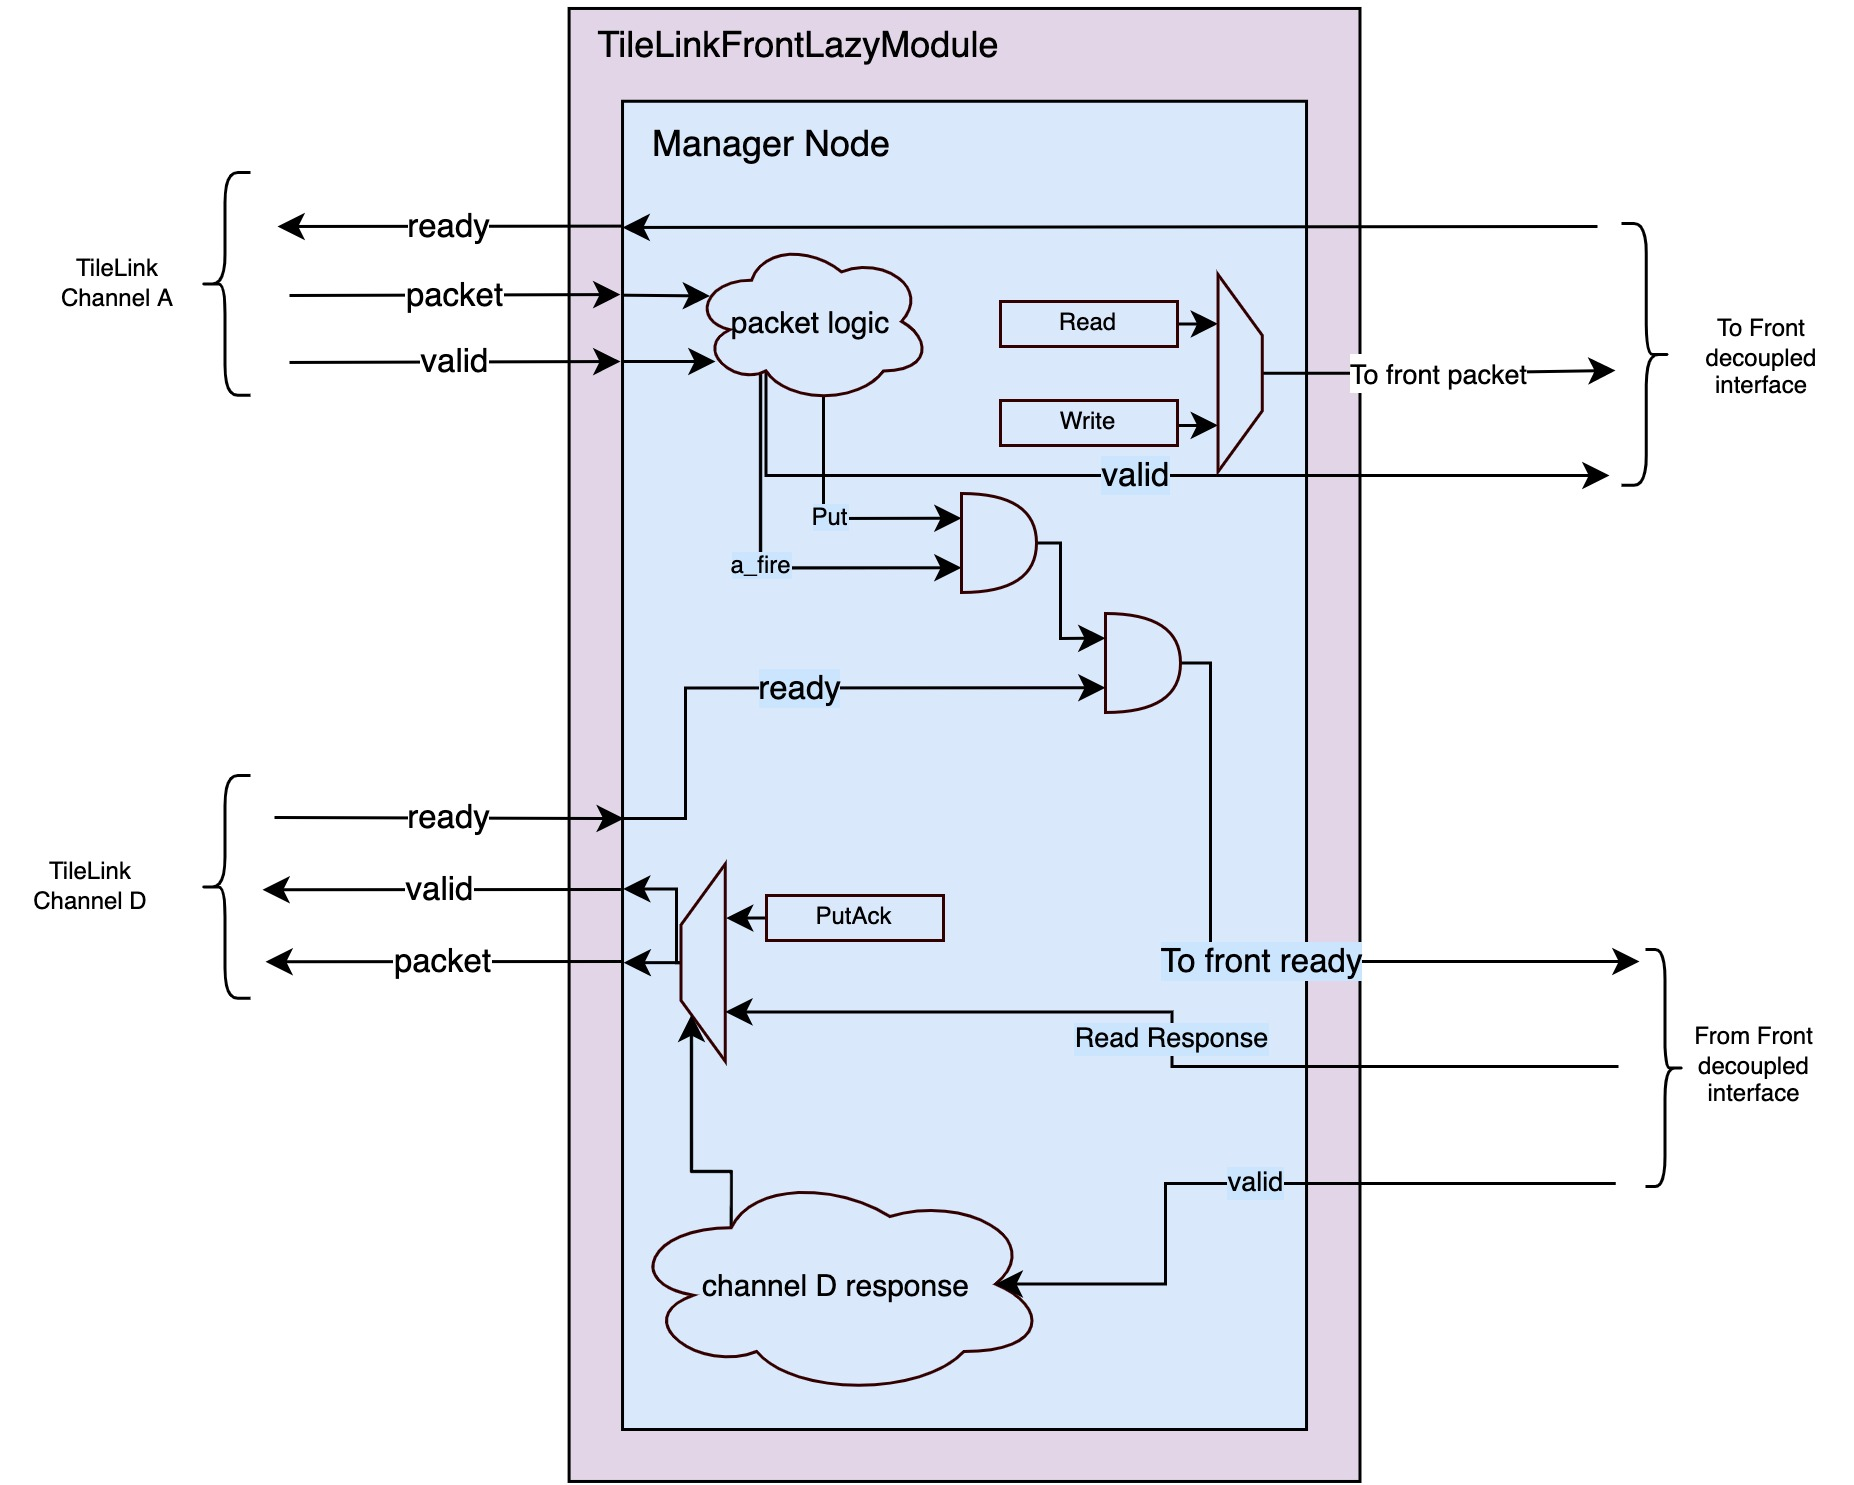
\includegraphics[scale=0.18]{images/tl-front.jpg}
    \caption{TileLink interface.}
    \label{fig:tli}
\end{figure}

A code snippet that instantiates the manager node with the parameters provided to the DDDR configuration case class is shown below. Some of the important parameters are the base address, region type, and beat byte. The beat bytes variable indicates the data width for each cycle of the transfer. Region Type of uncached indicates that the data has not been yet cached and the agent that requested this data needs to cache it. 
\begin{verbatim}
val device = new SimpleDevice("ddr-front", Seq("ddr,ddr0"))
val beatBytes = tlParams.BEATSIZE / 8
val node = TLManagerNode(Seq(TLSlavePortParameters.v1(
    Seq(TLSlaveParameters.v1(
      address = Seq(AddressSet(tlParams.ADDRESS, tlParams.SIZE)),
      resources = device.reg,
      regionType = RegionType.UNCACHED,
      executable = true,
      supportsGet = TransferSizes(1, beatBytes),
      supportsPutFull = TransferSizes(1, beatBytes),
      supportsPutPartial = TransferSizes(1, beatBytes),
      fifoId = Some(0))),
    beatBytes = beatBytes)))
\end{verbatim}

The TileLink module captures the requests arriving through the A channel. These requests are then determined to be either a write or read request based on the packet header and opcode bits. Every write request is responded to with an acknowledgment on the D channel immediately. The acknowledgment of the put requests establishes that the put request has been registered by this agent. The read requests are responded to after the data is read from the device and is ready to be sent to the requesting agent in the system. The logic in the TileLink module needs to translate the TileLink standard packets to an internal protocol bundle as shown below. 
\begin{verbatim}
class FrontToDP extends Bundle {
  val isWrite       = Output(Bool())
  val data          = Output(UInt((geom.TOTALBITS).W))
  val address       = Output(UInt((geom.FULLADDRBITS).W))
  val byteEnable    = Output(UInt((geom.TLBYTEEN).W))
  val requesterID   = Output(UInt((tlParams.RIDW).W))
  val bankNo        = Output(UInt(3.W))
}
\end{verbatim}
Once the responses to the read commands are ready, the memory controller datapath transfers the data to the TileLink module using the bundle shown below. 
\begin{verbatim}
    
class DataPacket extends Bundle {
  val hw            = Output(Vec(geom.TOTALBITS/dfi.DWIDTH, UInt(dfi.DWIDTH.W)))
  val requesterID   = Output(UInt((tlParams.MASTERIDSIZE).W))
}
\end{verbatim}
The hw field in the DataPacket corresponds to half-word data fields. A total of 256 bits of data is retrieved from the memory and is concatenated together as half-word data fields in this packet. The memory controller front-end logic guarantees an in-order response to the read requests. This needs to be handled by the datapath since the memory controller core might issue the requests to separate banks out-of-order. Every read transaction that is ready to be sent out to the SoC must go through the TileLink module logic. The internal packets are then translated to TileLink AccessAckData responses.
\section{Asynchronous Crossing}
The memory controller must adhere to a specific speed bin determined by the JEDEC specification. This frequency determines the frequency of the memory controller and the PHY. In this project, we targeted a frequency ratio of 1:4 between the memory controller and the PHY. This frequency ratio gives rise to 1:4 mapping commands from the memory controller to the clock phases of the PHY. In addition, the SoC might be running at a much higher frequency than the memory controller. To perform a clock domain crossing we have placed an asynchronous FIFO in between the TileLink module and the datapath of our design. The block diagram in Figure \ref{fig:cdc} shows the crossing point between the SoC domain and the controller domain. 

To determine the queue size for the asynchronous FIFO, a sampling frequency on the consumer side, and a producing frequency is needed. Given a frequency ratio of 2 to 1 from SoC to MC and assuming the worst-case scenario of en-queuing transactions with MC not ready:\\
    \indent SoC frequency = 800 MHz \\
    \indent MC frequency = 200 MHz \\
    \indent Burst Length = $b$ requests\\
    \indent Maximum enqueue frequency = $1 \frac{request}{cycle} * \frac{800 cycles}{1 s} = 800 \frac{requests}{s}$\\
    \indent Total time to write $b$ requests = $\frac{b}{800} s$\\
    \indent Maximum dequeue rate = $1 \frac{request}{cycle} * 200 \frac{cycles}{s} = 200 \frac{requests}{s}$\\
    \indent Maximum number of dequeues during the burst = $\frac{b}{800} s * 200 \frac{requests}{s} = \frac{b}{4} requests$\\
    \indent Number of transactions to be stored in the queue = $b - \frac{b}{4} = \frac{3b}{4}$\\
    
With the burst length of $b$ and 800 MHz frequency to a 200 MHz frequency, we would need to have a buffer depth of $\frac{b}{4}$. In addition, a designer needs to perform workloads and simulate the design at the system level to understand the depth necessary such that the FIFO would not become the bottleneck of the system.

\begin{figure}[h]
    \centering
    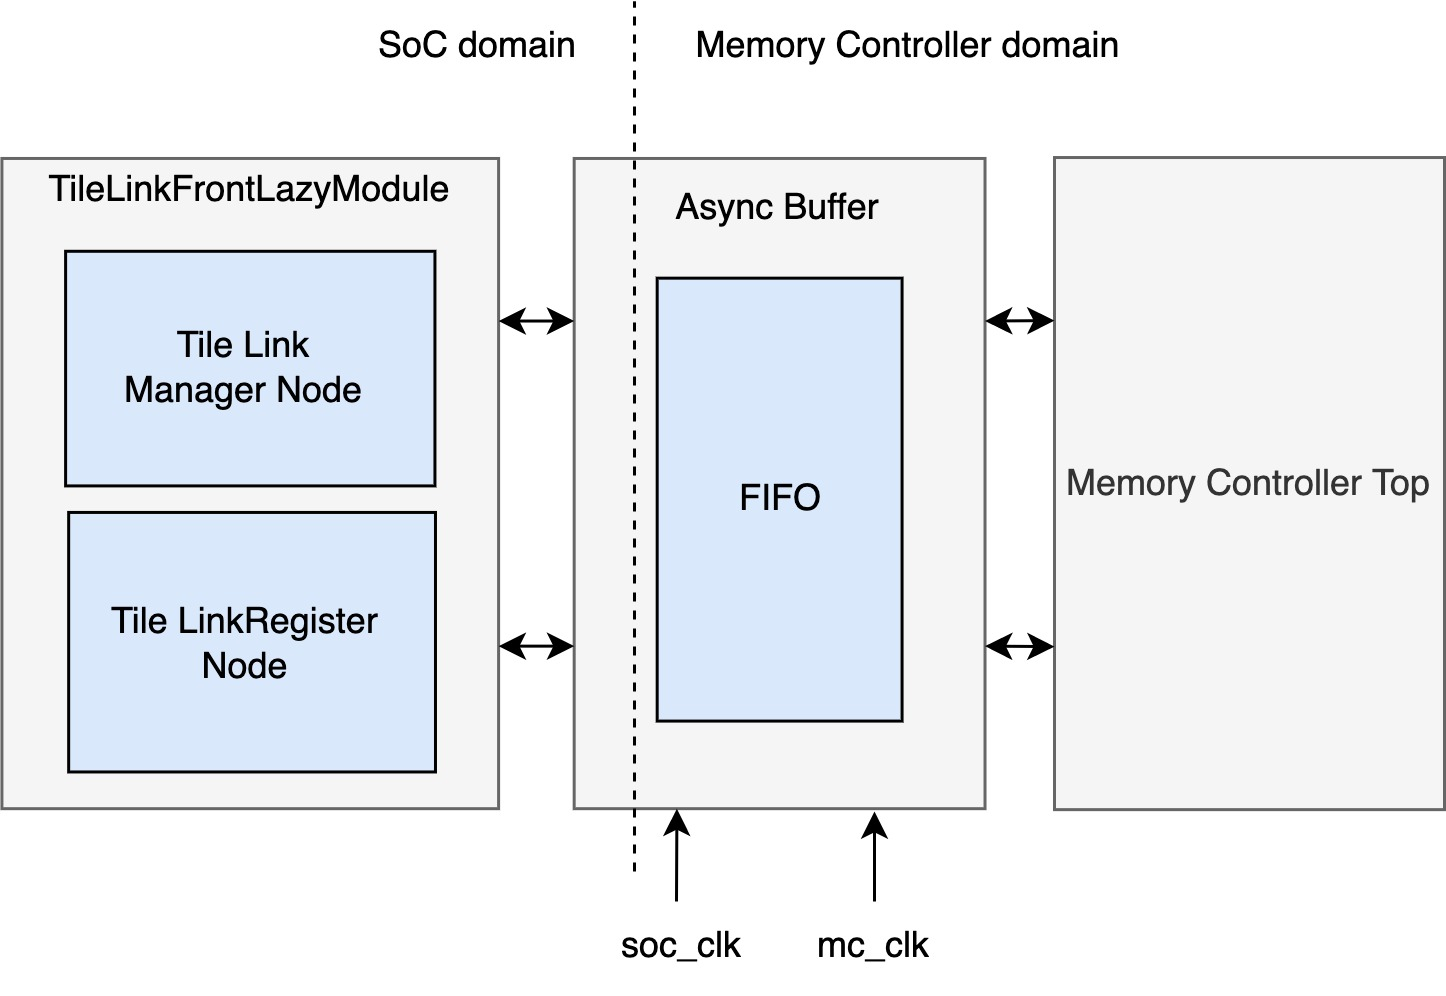
\includegraphics[scale=0.2]{images/cdc.jpg}
    \caption{Asynchronous crossing.}
    \label{fig:cdc}
\end{figure}
\newpage
\section{Controller Datapath}
The memory controller datapath takes in read and writes packets that are passed by the TileLink module. These packets have an internal format and are processed in the controller datapath. \footnote{The architecture planning and design of this unit in the design were done by Ken and me. The implementation of the sub-modules was a shared effort by Ken Ho and me.} 

The memory controller datapath contains ID assignment logic and dispatching logic to bank machines. In addition, the datapath has ports to insert data into the internal read and write queues. The datapath covers the read and writes queues units; the datapath is connected to two different points of the design, the front-end TileLink module, and the DFI module. DFI is a protocol specification to bridge between the controller and the PHY \cite{dfi}. The datapath is also responsible for changing the addressing scheme to DRAM-specific addressing. TileLink addresses must then be sliced into the bank address, row address, and column address which are all defined by the DDR device capacity and organization. The bank address must be from 0 to 7 and requires 3 bits of the address. In order to interleave the requests among different banks, we dedicated 3 bits of the address between the column and row addresses. Row address spans a larger number of bits of the address and is also dependent on the target DDR device and capacity. Column address takes up the lower bits of the address to slice into the rows and select a subset of bits from the row buffer. A breakdown of the physical addresses is shown in Figure \ref{fig:addr}.
\begin{figure}
    \centering
    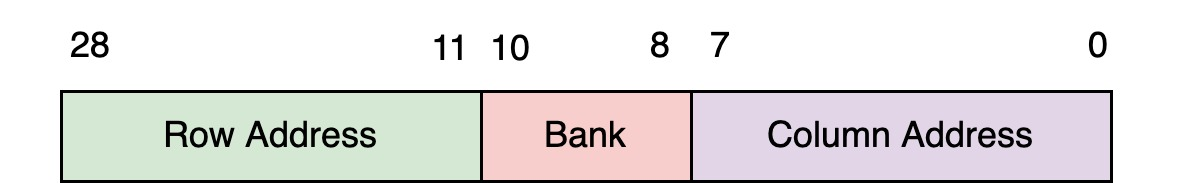
\includegraphics[scale=0.3]{images/address.jpg}
    \caption{Breakdown of physical address.}
    \label{fig:addr}
\end{figure}

Assignment of an ID to each transaction as they enter the controller is required for further referencing the transaction. As an example, a PUT transaction is entered into the datapath and is given a transaction ID. Furthermore, it enters the write queue where the data and transaction IDs are stored in an SRAM. Once the core logic processes the transaction and timing parameters are checked, the request can cross the controller and PHY interface. At this stage, the write data needs to be sent out to the PHY as well as the control signals. The transaction is identified using the previously assigned ID and is retrieved from the SRAM to be sent to PHY. A similar procedure applies to a read transaction that enters the controller. Once a read transaction enters the datapath, an ID is assigned to the transactions. A bundle with the necessary metadata is then stored in the read queue for further processing of the read transaction. Once the read transaction is processed and the data is retrieved from the device, the read queue is referenced, and both the data and transaction metadata are stored in the read SRAMs. The ID can also be used to identify the relative age of a pending transaction in the queues as the ID generation is an incremental counter. 

The bank machines internal queues and the main transaction queue control the ready signal outputted from the datapath. The ready signal is then translated and connected to the asynchronous FIFO which in turn exposes another ready signal to the TileLink module. Once the ready signal is low, the senders in the SoC would need to re-try sending their packets. The TileLink module in the design takes the responsibility of receiving TileLink messages over channel A and sending them back over Channel D as mentioned in section 2.2.
\subsection{Transaction Queue}
A main transaction queue is used to store the requests as they enter the datapath. The queue is also used to provide a ready signal to the asynchronous FIFO and the TileLink module. The metadata and the transaction itself are stored in the queue. The transaction fields and metadata are write enable (we), address (addr), ID (cmdID), mask (byteEnable), bank (bankNo), and requester ID shown below:
\begin{verbatim}
class BankInPacket (val geom : GeomParams) extends Bundle {
  val we            = Output(Bool()) // write enable
  val addr          = Output(UInt((geom.FULLADDRBITS).W))
  val cmdID         = Output(UInt((geom.IDBITS).W))
  val byteEnable    = Output(UInt((geom.TLBYTEEN).W))
  val bankNo        = Output(UInt(3.W))
  val requesterID   = Output(UInt(tlParams.MASTERIDSIZE.W))
}
\end{verbatim}
\subsection{Read Queue}
The read queue module contains the read queue with the corresponding SRAMs and a read in-order queue for enforcing the ordering of read responses. 

The purpose of having a read-in-order queue is to guarantee the same ordering of read responses to the system as the memory controller received. A usual optimization is to avoid such guarantees; however, having this scheme allows us to keep track of transaction processing times, and quality of service at a system or NoC level. 

The read transactions enter the read-in-order queue as they enter the read queue module. Similarly, the data that was previously requested by the controller to the DRAM device can be inserted into the read SRAMS at any cycle that the data is received by the controller. Once the SRAM row is filled with the requested data, the row is set to be filled using a per-row bit vector. On every cycle, if there exists a pending read transaction in the read-in-order queue and the data corresponding to that transaction is available in the read SRAMs, the transaction at the top of the queue is dequeued. The dequeued read transaction is the oldest pending transaction with ready data available in the read SRAMS.

The read queue contains eight SRAM banks in parallel providing a total of 256 bits wide data. The depth of the SRAMs is parameterized by the designer; however, the depth of the SRAMs determines whether or not the controller can issue a read command. A one-bit valid signal per row is used to indicate if the row is empty or allocated. An allocate request is issued to the module by the datapath once the read transaction is entered into the datapath. The read transaction allocates a row in the SRAM and enqueues the transaction into the read in-order queue. Once the data is received by the DFI module, the 256-bit wide data is entered into the previously allocated SRAM row. The address of the SRAM row is determined using a Content Addressable Memory table (CAM table). The data is then stored in the allocated SRAM row using the address found from the CAM. Transaction IDs are used to compare and find the addresses from the CAM table. A block diagram of the read queue is depicted in Figure \ref{fig:reqdq}. 

The designer of the SoC should configure the depth of the queues appropriately and pay attention to the maximum allowable pending transaction. It is very important to note that a read transaction that is serviced and responded to by the DRAM device enters the controller and is captured by the logic in the read queue and the SRAMs. As a result, if a read transaction that is at the head of the read-in-order queue enters the pipeline, it will not be sent to the SoC immediately as a read and write to an SRAMs row must not occur on the same cycle.

In the case of lower-depth queues, a designer may choose to avoid SRAMs and map the memory logic to register-based memory banks.
\begin{figure}[H]
    \centering
    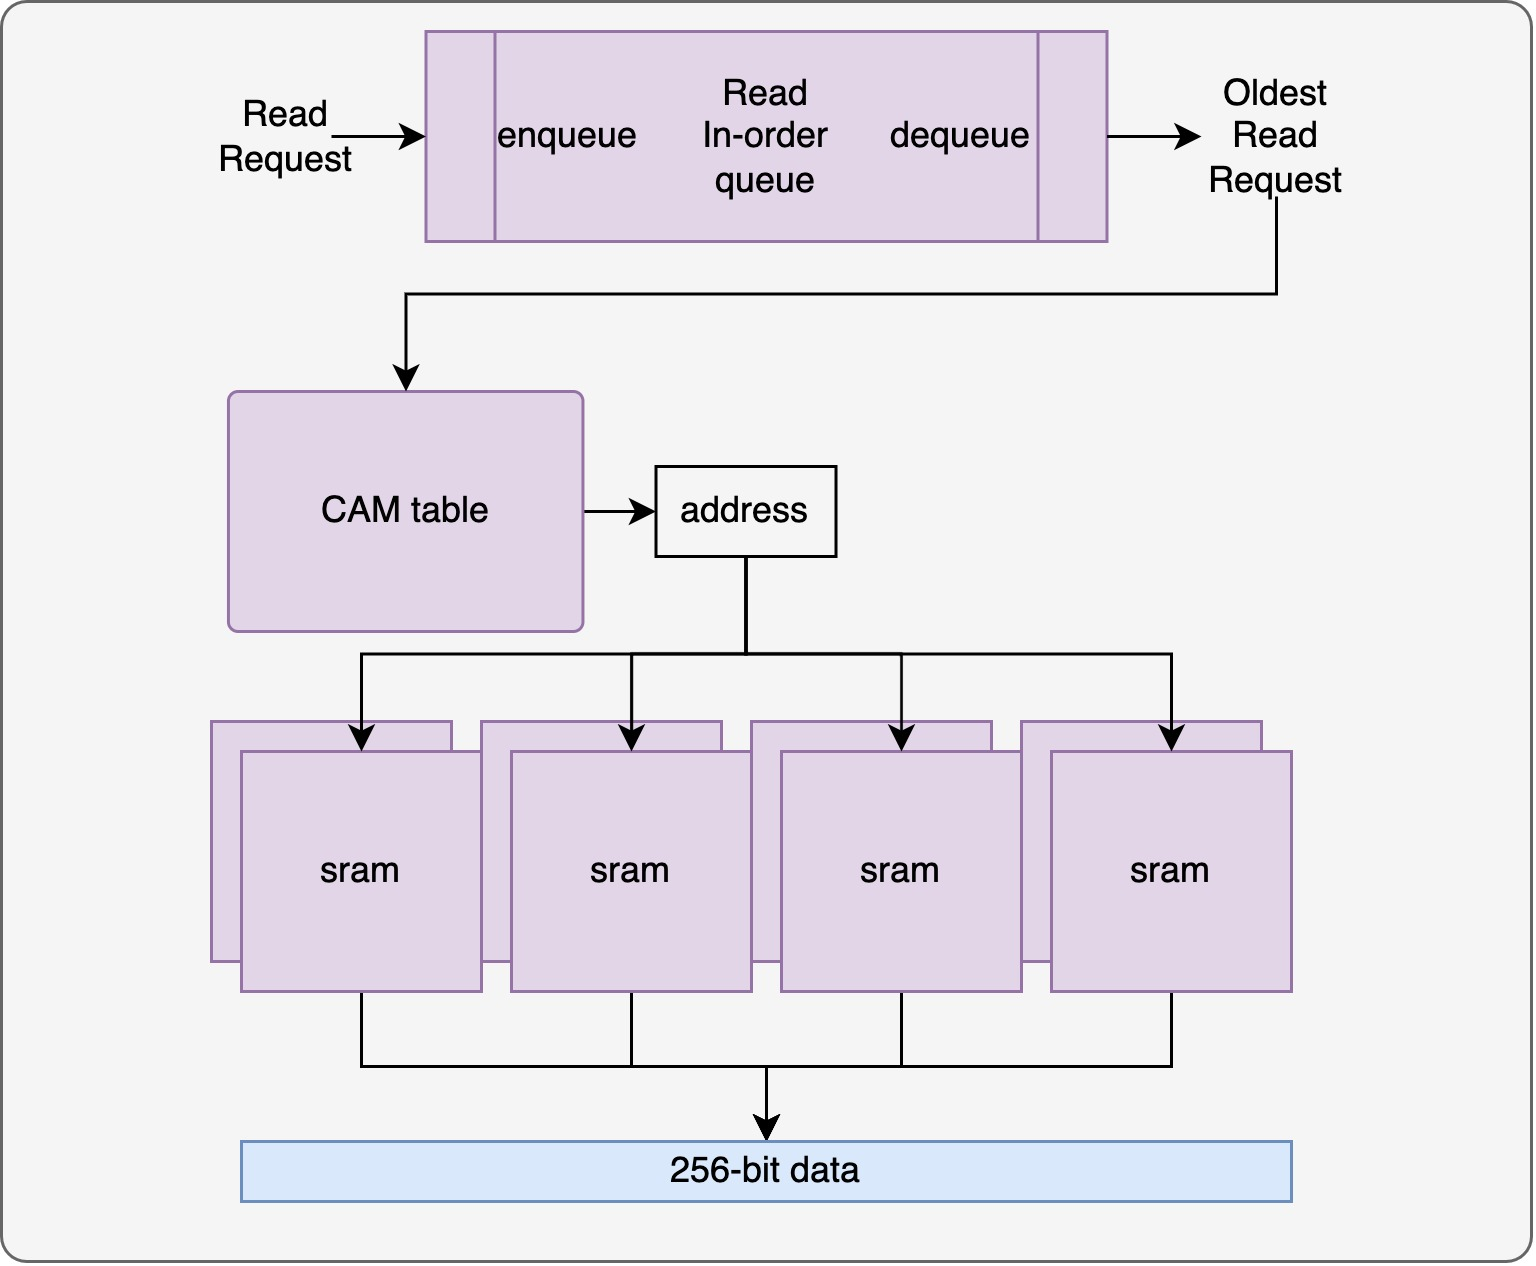
\includegraphics[scale=0.2]{images/readQ.jpg}
    \caption{Read queue.}
    \label{fig:reqdq}
\end{figure}
\subsection{Write Queue}
Similar to the read queue, a module is dedicated to keeping the write transactions within the datapath until the write transaction is processed and ready to be issued to the PHY interface. 
The write queue contains eight SRAMs to store a total of 256 bits of data internally. Every write transaction enters the write queue; the data corresponding to the write with the ID of the transaction is stored in an empty row of the write SRAMs. The address of the SRAM row is stored in a CAM table that is accessed in the future using the transaction ID. A high-level block diagram of the write queue is shown in Figure \ref{fig:wrQ}.
\begin{figure}
    \centering
    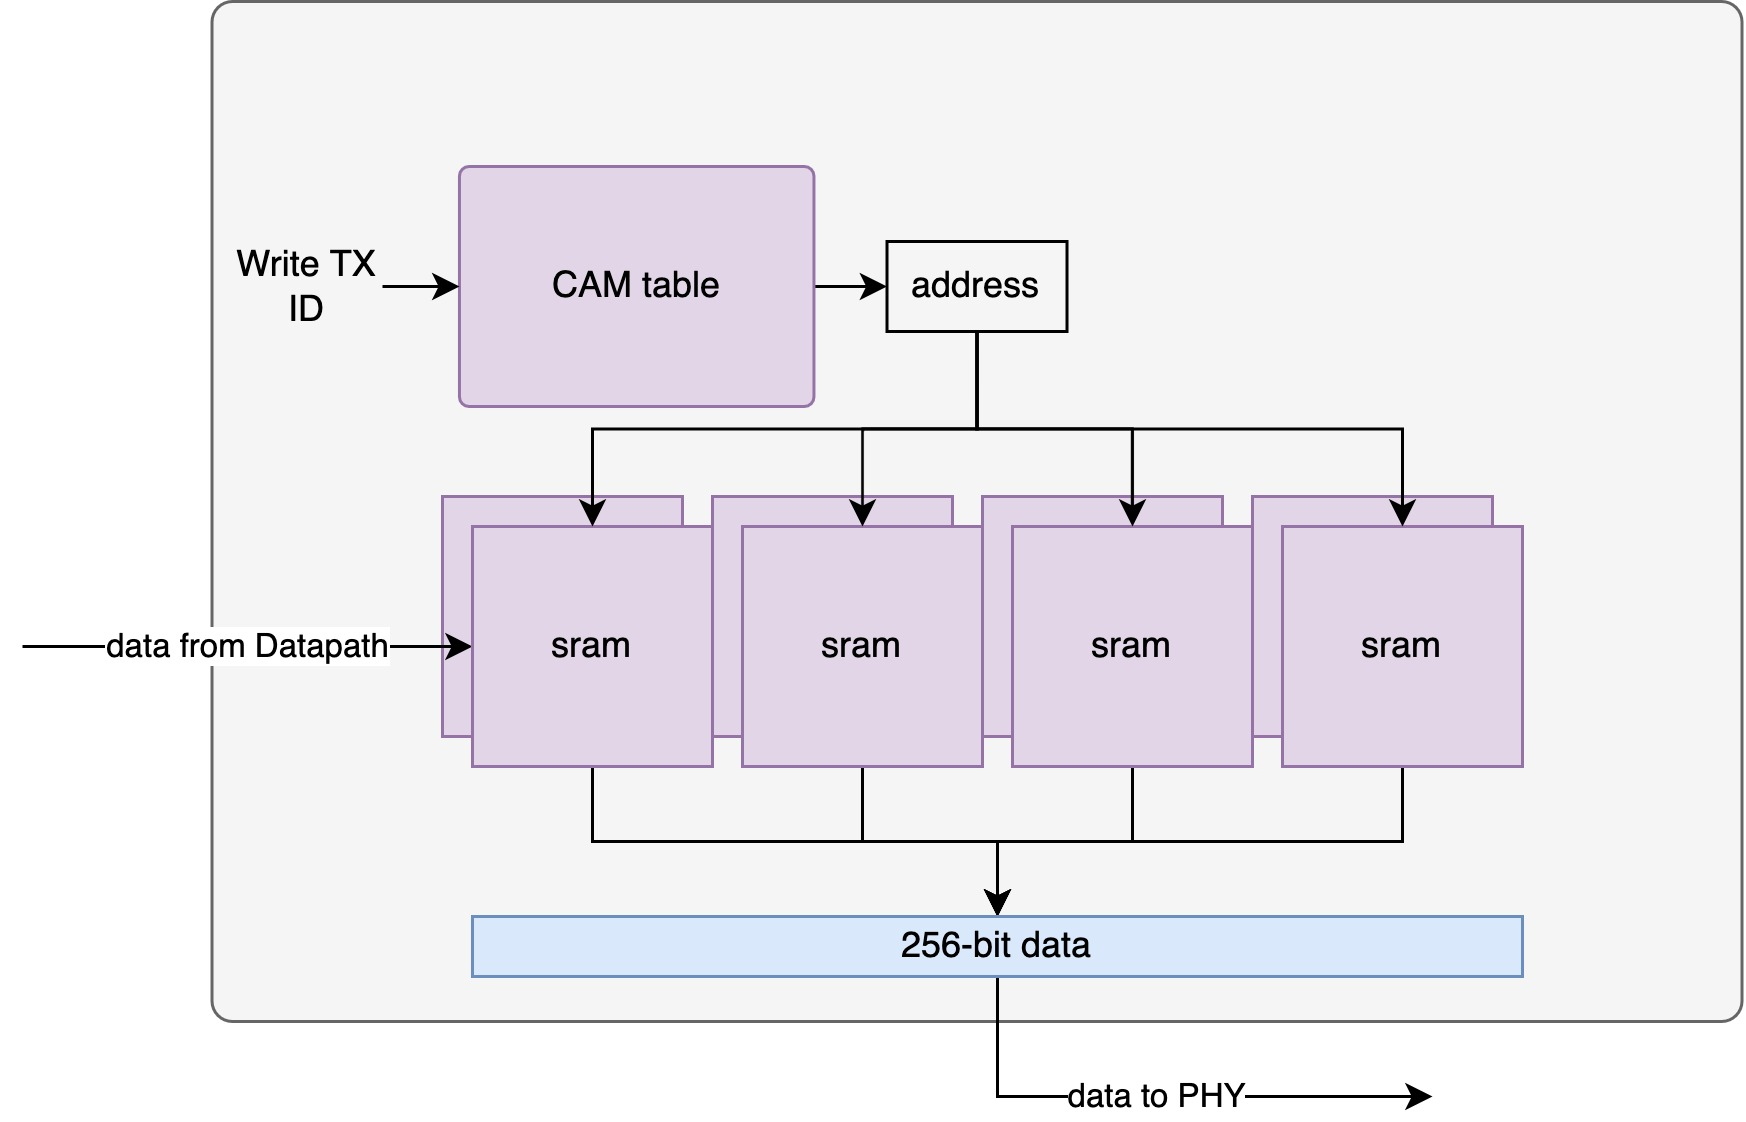
\includegraphics[scale=0.2]{images/wrQ.jpg}
    \caption{Write queue.}
    \label{fig:wrQ}
\end{figure}
\section{Bank Machines}
The controller core contains eight Bank Machine modules each of which keeps track of the state of a bank in one rank of the DRAM device. A diagram of the FSM that each bank machine implements is shown in Figure \ref{fig:fsm}. \footnote{The architecture planning of this unit was a shared effort by Ken Ho and me. Implementation of this unit referenced LiteDRAM implementation \cite{enjoydigital}. Verification of the unit was done by Ken Ho.
}

A bank machine implements the JEDEC state machine for each bank with the additional functionality of ensuring the timing parameters are met. 
A memory transaction is split into at least two commands each of which has its own timing parameters. Table \ref{tab:cmd} shows a summary of the commands that the memory controller needs to issue. A read transaction to an address that was not read by the controller recently must issue a row activate command to the device first. The row activate command (RAS) is issued to the device so that the word line corresponding to the address is activated and the content of the row is sensed and registered into the row buffer. A read or a write command is considered a column access command (CAS). This command requires us to wait for TRCD parameter, which is some number of cycles specified by JEDEC specification. Another important timing parameter is TCCD which denotes the delay between two consecutive column access commands. For the read transaction to be safely issued to the device, all the relevant parameters must be checked beforehand. A legal command then can be issued to the device. 

A timing controller in the design refers to a counter that is restarted with the same value for each timing parameter. The timing parameters can be set using the TileLink register node. A core can be used to write data into a specific register that is mapped to a timing parameter. In an ASIC design, this gives the designer flexibility to modify a timing parameter at the time of the chip bring-up. In Figure \ref{fig:fsm}, a simplified version of the JEDEC state machine is shown. The bank machines have internal counter controllers for each timing parameter in addition to implementing this FSM.

The ordering of each command is specified by this FSM. However, there are additional queues in the bank machines in order to compare multiple transaction addresses to keep a row active in case of a hit. This optimization can be further used to re-order transactions in the queues such that we can perform multiple CAS commands on the same activated row. This reduces the overhead of RAS commands. 
\begin{table}
    \centering
    \begin{tabular}{c|c}
        Command & Description \\
        \hline
        Activate & Row access, Activates a row\\
        Read & Column access, reads a subset of the row\\
        Write & Column access, writes to a subset of the row\\
        Precharge & Precharges the row to an idle state\\
        Auto-precharge & Automatic precharge after a read or write\\
        Refresh & Refreshes the bank to preserve the data\\
        Refresh all & Refreshes all the banks\\
        Precharge all & Precharges all the banks, all go to idle state
    \end{tabular}
    \caption{LPDDR4X standard commands.}
    \label{tab:cmd}
\end{table}

\begin{figure}
    \centering
    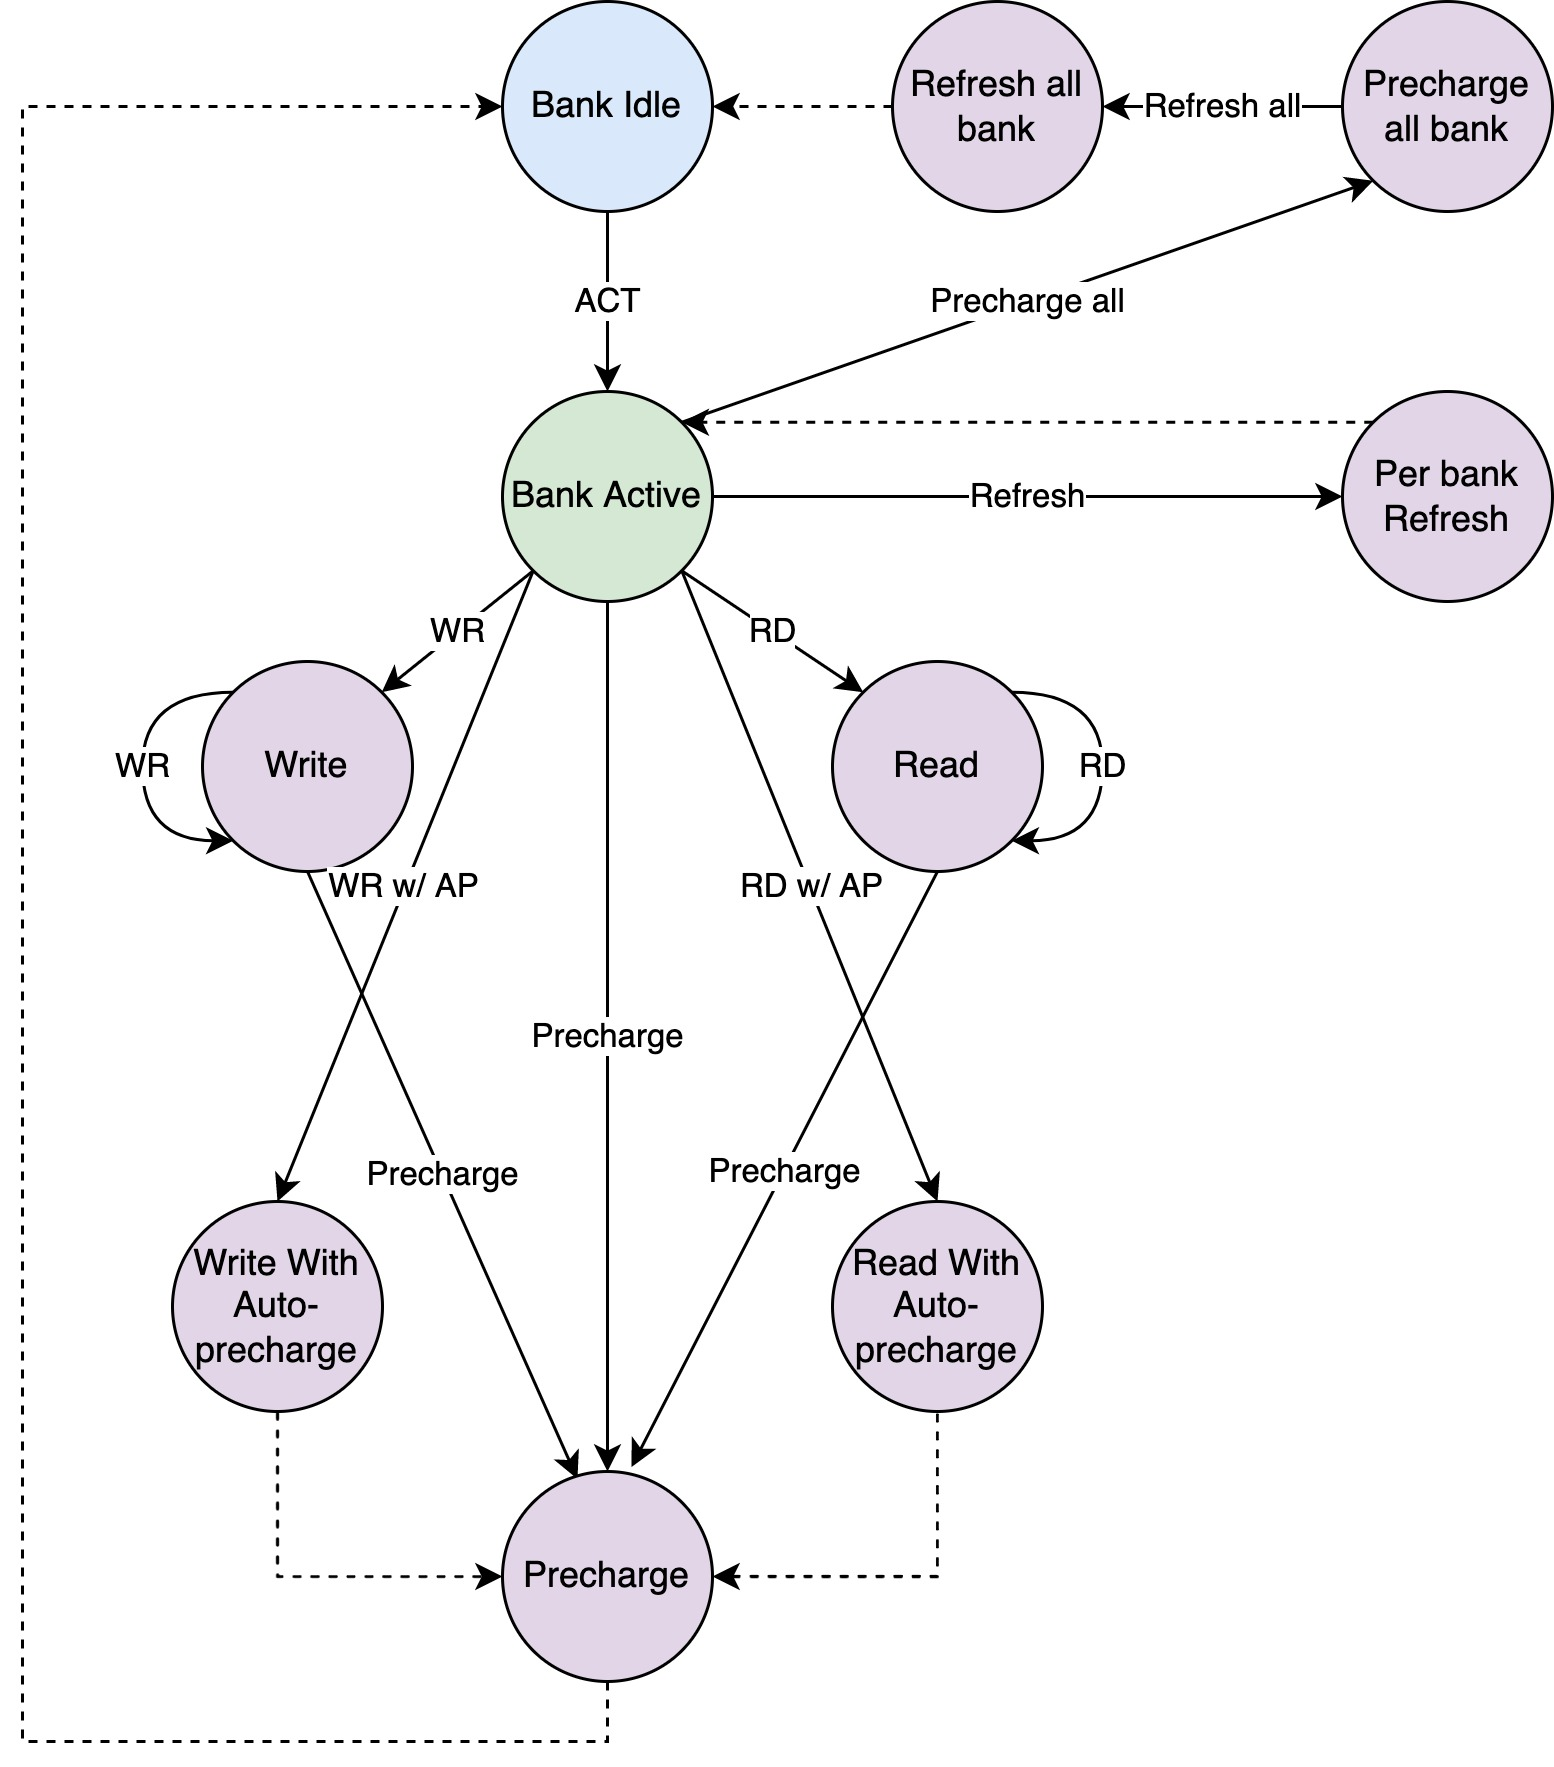
\includegraphics[scale=0.2]{images/fsm.jpg}
    \caption{Per bank state machine.}
    \label{fig:fsm}
\end{figure}

\section{Refresh Controller}
A refresh is needed to maintain the logical value of a bit-cell. This operation is mandatory and due to the leakage of charge from the trench capacitors of the memory cells. A separate controller module is responsible for refreshing the DRAM device. A compatible LPDDR4X memory device can refresh banks individually, or all the banks at the same time. In our design, we have a refresh controller that refreshes all the banks by first issuing a precharge-all command. The precharge-all command must be issued before a refresh since a bank must be in an idle state before a refresh operation. The refresh controller has a counter internally to maintain a timely refresh to the device. TREFI is specified as the average refresh interval with a value of 3.904 microseconds. A counter that counts the number of cycles up to TREFI sends a refresh request to the multiplexer module. Once the request is approved by the multiplexer, the refresh controller takes over the command bus and can start issuing commands. The acknowledgment from the multiplexer is necessary since the multiplexer module ensures that bank machines transition to the idle state. Figure \ref{fig:refall} show an example of the refresh procedure and commands to be sent by the refresh controller. 
\newpage
The first phase for a refresh sequence is to issue a DFI standard command for pre-charge all as below:
\begin{verbatim}
          cmd(0).dfiCs := true.B
          // Precharge-1 Low (default)
          // Precharge-2 Hi
          cmd(2).dfiAddress := "b11_0000".U
          cmd(2).dfiCs := true.B
          // Precharge-2 Low
          cmd(3).dfiAddress := "b00_0000".U
          cmd(3).dfiCs := false.B
\end{verbatim}
\begin{figure}
    \centering
    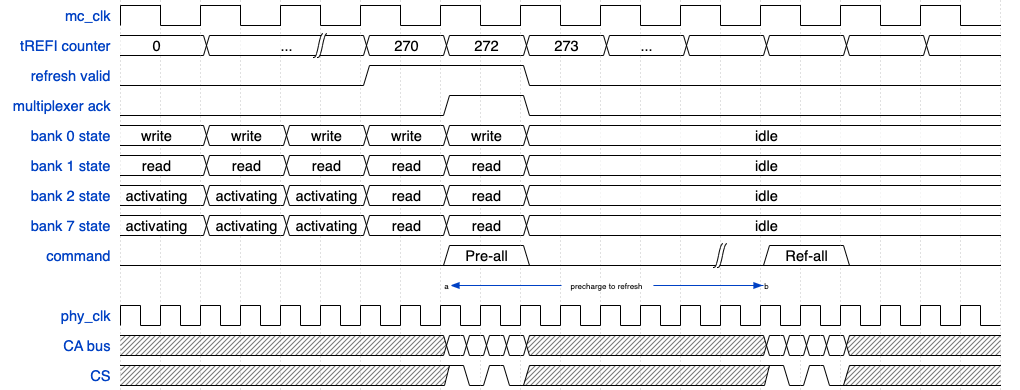
\includegraphics[scale=0.5]{images/refresh-wave.png}
    \caption{Refresh-all sequence.}
    \label{fig:refall}
\end{figure}
The commands are sent over in one cycle of the memory controller; however, each command will be translated into four cycles of DFI clock domain. Each command can be split into four phases of the controller cycle and sent out as a vector of size four. The dfiAddress field in the code snippet above maps to the CA bus which is the command and control bus of the channel. 
\section{Controller Bring-up}
At the time of bring-up, the DDR module in the chip must be configured with the timing parameters and mode register values.

The sample code below shows the timing parameters that need to be configured at the time of bring-up. The configuration is done using the TileLink register node and is done by a core in the system issuing writes to the corresponding address.
\begin{verbatim}
val tphycwl = RegInit(8.U(timeBits.w.W))
val tphycl = RegInit(14.U(timeBits.w.W))
val twr = RegInit(4.U(timeBits.w.W))
node.regmap(
      0x00 -> Seq(RegField(timeBits.w, tphycwl)),
      0x01 -> Seq(RegField(timeBits.w, tphycl)),
      0x02 -> Seq(RegField(timeBits.w, twr)),
      ...)
\end{verbatim}

A bare-metal software can be written to write the timing registers and the device mode registers. 

\section{Scheduling Logic}
The scheduling logic determines which request from each bank can be issued to the device at any cycle. The Bank Machines provide a command that meets the per bank timings to the \verb|CommandChooser| module, where a round-robin arbiter provides an index to pick the next command to be sent. \verb|CommandChooser| module can be optimized to use more sophisticated arbiters to optimize for DQ bandwidth. In addition, a fairer history-based arbiter can be deployed in place of the round-robin arbiter. \footnote{The architecture planning for this unit was done by Ken Ho and me. The implementation of the scheduling logic was done by Ken Ho.
}

\subsection{Open-page Policy}
In an open-page policy mode, the Bank Machines can keep a row open after an activate and a CAS command. Further CAS commands can be issued after a CAS to CAS latency. Open-page policy avoids an activation for the second CAS command. Our design incorporates this idea into the Bank Machine as a configurable parameter. If configured to perform an auto-precharge command, a CAS command automatically performs a precharge and puts the bank in an idle state. However, if not set to use auto-precharge, the look-ahead command buffer in the Bank Machine allows us to check for a row hit. A row hit follows by keeping the row open and issuance of the second CAS command right after. 

A concerning side effect of the open-page policy is the potential starvation of other requests to the same bank in case a row is being accessed regularly. This could be due to an application performing reads and updates to a specific variable or a malicious code accessing one particular variable in a loop to exploit the open-page policy.



\section{Controller Configuration}
Three main case classes are used to configure the LPDDR4 controller based on the design of the SoC and memory system. 

The Geometry class corresponds to the DRAM device configuration, time counter width, depth of the queues in the design, row slice from the address, column slice, and bank slice. This case class can be instantiated in the configuration class of the chip. 

DFI parameters case class corresponds to the DFI-specific parameters used in the design. DFI width, the number of phases per controller clock, and PHY slice widths are all determined in this case class. Similar to the Geometry class, the DFI parameters should be instantiated and modified per design-specific constraints. 

A TileLink parameter case class is also needed to configure the TileLink nodes needed in the design. This case class requires the designer to provide two base addresses. One address for the base of the DRAM. This address should be the base of the memory for the SoC and must be a cachable address range. The other base address is used for the register node and configuration of the timing parameters. The configuration base address can be associated with a control address and should be uncachable. 

The DDR generator has a \verb|CanHaveMasterTLDDRPort| trait. This trait is used as one of the traits that \verb|DigitalChip| inherits. Once added to the \verb|DigitalChip| of Chipyard, the trait instantiates the TileLink module and connects the internal TileLink node for memory to the memory bus of the system. It also connects the internal register node in the TileLink module to the periphery bus of the system. The trait instantiates the DDR top module and connects the interfaces of the top module to the TileLink module. The connection must happen in this way due to TileLink requirements for elaboration and TileLink lazy module system.
\begin{verbatim}
class DigitalTop(implicit p: Parameters) extends ChipyardSystem
    with ddr.CanHaveMasterTLDDRPort

        
class WithDDR(val geom: GeomParams, val dfi: DFIParams, val tl:  TileLinkParams) 
    extends Config((site, here, up) => {
  case DDRKey => Some(DDRParams(geom = geom, dfi = dfi, tl = tl))
})  
\end{verbatim}

A chip configuration with the LPDDR4 memory controller would add \verb|WithDDR| with the intended parameters to instantiate the controller. 


\chapter{Micro-architecture}
We have designed and written the RTL in Chisel \cite{10.1145/2228360.2228584} domain-specific language or DSL. Chisel is a DSL embedded in Scala programming languages. It allows for easy integration to Chipyard for different purposes such as FireSim \cite{8416816} simulations, VLSI integration, and FPGA targets. 
\section{Chisel API}
The APIs are implementation of common hardware constructs provided to us by Chipyard \cite{chipyard} and Chisel \cite{Asanović:EECS-2016-17} and the team of Chipyard developers.

We have used Chisel constructs in our design to implement common hardware blocks. A queue is an example of such constructs that are provided by Chisel. 
\begin{verbatim}
val reqQueue = Module(new Queue(new MainQueue(geom, tlParams),
                                geom.QUEUEDEPTH, pipe=false))    
\end{verbatim}
The code above instantiates a simple queue that stores the requests entering the memory controller data path. The reqQueue elements then can be accessed using the I/O ports of the Queue module. The Queue module provides a ready-valid interface on both enqueue and dequeue sides. When there is a new request, the request bundle can be stored using the API as shown below:
\begin{verbatim}
    when (io.frontReq.fire) {
      reqQueue.io.enq.valid := true.B
      reqQueue.io.enq.bits.we := io.frontReq.bits.isWrite
      reqQueue.io.enq.bits.addr := io.frontReq.bits.address
      reqQueue.io.enq.bits.cmdID := id
      reqQueue.io.enq.bits.bankNo := io.frontReq.bits.bankNo
      reqQueue.io.enq.bits.byteEnable := io.frontReq.bits.byteEnable
      reqQueue.io.enq.bits.requesterID := io.frontReq.bits.requesterID
    }
\end{verbatim}

The when construct corresponds to a combinational logic always block in Verilog. The code above uses methods defined in the IO class such as fire. Fire is the event that both ready and valid are high for an interface. This style of coding makes it easier and faster to write the RTL. 

Using standard Scala functional programming features such as \verb|.filter()|, \verb|.foreach()|, and \verb|.tabulate()| helped us write the RTL more concisely while maintaining code readability. 

Packets in Chisel can be constructed by creating a class that extends the Bundle class of Chisel. A bundle is a group of directional wires that have the same context. In our case, we standardized all of our bundle classes to contain output wires. In case a bundle is used as an input to a module, a \verb|Bundle| can be used to flip all the directions for that bundle. An example bundle usage in our RTL is the input to the Bank Machines described in Chapter \ref{chap:arch}. The bank input packet includes a field for write or read, address, id, and mask. If the transaction is a write transaction, the write enable field or \verb|we| is true and the byte enable is used to mask the write data. 
\begin{verbatim}
class BankInPacket (val geom : GeomParams) extends Bundle {
  val we         = Output(Bool())
  val addr       = Output(UInt((geom.FULLADDRBITS).W))
  val cmdID      = Output(UInt((geom.IDBITS).W))
  val byteEnable = Output(UInt((geom.TLBYTEEN).W))
}
\end{verbatim}
Using this bundle as an input port to the Bank Machine module is done through a Decoupled interface which adds ready and valid signals to the bundle. 
\begin{verbatim}
class BankMachine (val geom : GeomParams, val bankNo : Int) extends Module {
  val io = IO(new Bundle {
    val in = Flipped(Decoupled(new BankInPacket(geom)))
    ...
\end{verbatim}
The in field of the IO port in a Bank Machine is a decoupled, flipped bundle of \verb|BankInPacket|. The \verb|Decoupled| makes the IO port a decoupled interface with ready and valid signals. The ready signal is set by the consumer of this packet which is the Bank Machine module, and the valid signal is asserted by the producer of the signal which is the data path module. A \verb|io.in.fire| event corresponds to the transfer of the packet from the producer to the consumer. 
\section{Datapath Micro-architecture}
The datapath in our design refers to the module that takes in requests from the TileLink module and keeps track of the transactions and the data. As an example, a write request must be kept in the data path until the write transaction is ready to be issued to DFI. At that point, the data can be taken out of the memory controller and sent to the DFI. 
The data path has two main modules within it, a read queue module, and a write queue module. The read, and write queues keep the data in 8 banks of SRAMs.
The data path interfaces to the top module of the memory controller. The top module connects the ports from the data path to the DFI read and write interface. The top module connects the data path to its input ports which are connected to the TileLink front module. Figure \ref{fig:data_uarch} shows the micro-architecture diagram of the data path. The data path has an internal counter for ID assignment to transactions. This counter is by default a 10-bit counter but can be configured to a wider counter to avoid ID collisions. Each TileLink request that is captured by the TileLink module first is synchronized to the controller clock frequency and then enters the data path module where it is assigned an ID. If the transaction is a write transaction, then the data path must store the data with the corresponding ID in the write queue SRAMs. The depth of the write queue SRAMs indicates the maximum write requests that can be in flight at any point. However, the request queue which stores both read and write transactions provided a ready signal to the SoC. The designer of the SoC must size the request queue to be equal to or greater than the write or read queues. 

A capturing logic is implemented in the data path to capture a read response from the DFI. Once a read response arrives, the DFI packet asserts a read data valid signal. The data is delivered to DFI on PHY clock frequency which is four times faster than the controller clock. DFI delivers the data to the memory controller per cycle using four phase scheme. On each cycle, data is split into four phases of 32 bits that are delivered over 2 cycles which make up the 256-bit total data width of the controller. The read data capturing waveform is shown in Figure \ref{fig:read-cap}.

A similar logic is in place to stream the write data from a 256-bit wide register to the DFI over two cycles.  Figure \ref{fig:write-trans} shows the transmission of the write data to DFI. 
\begin{figure}
    \centering
    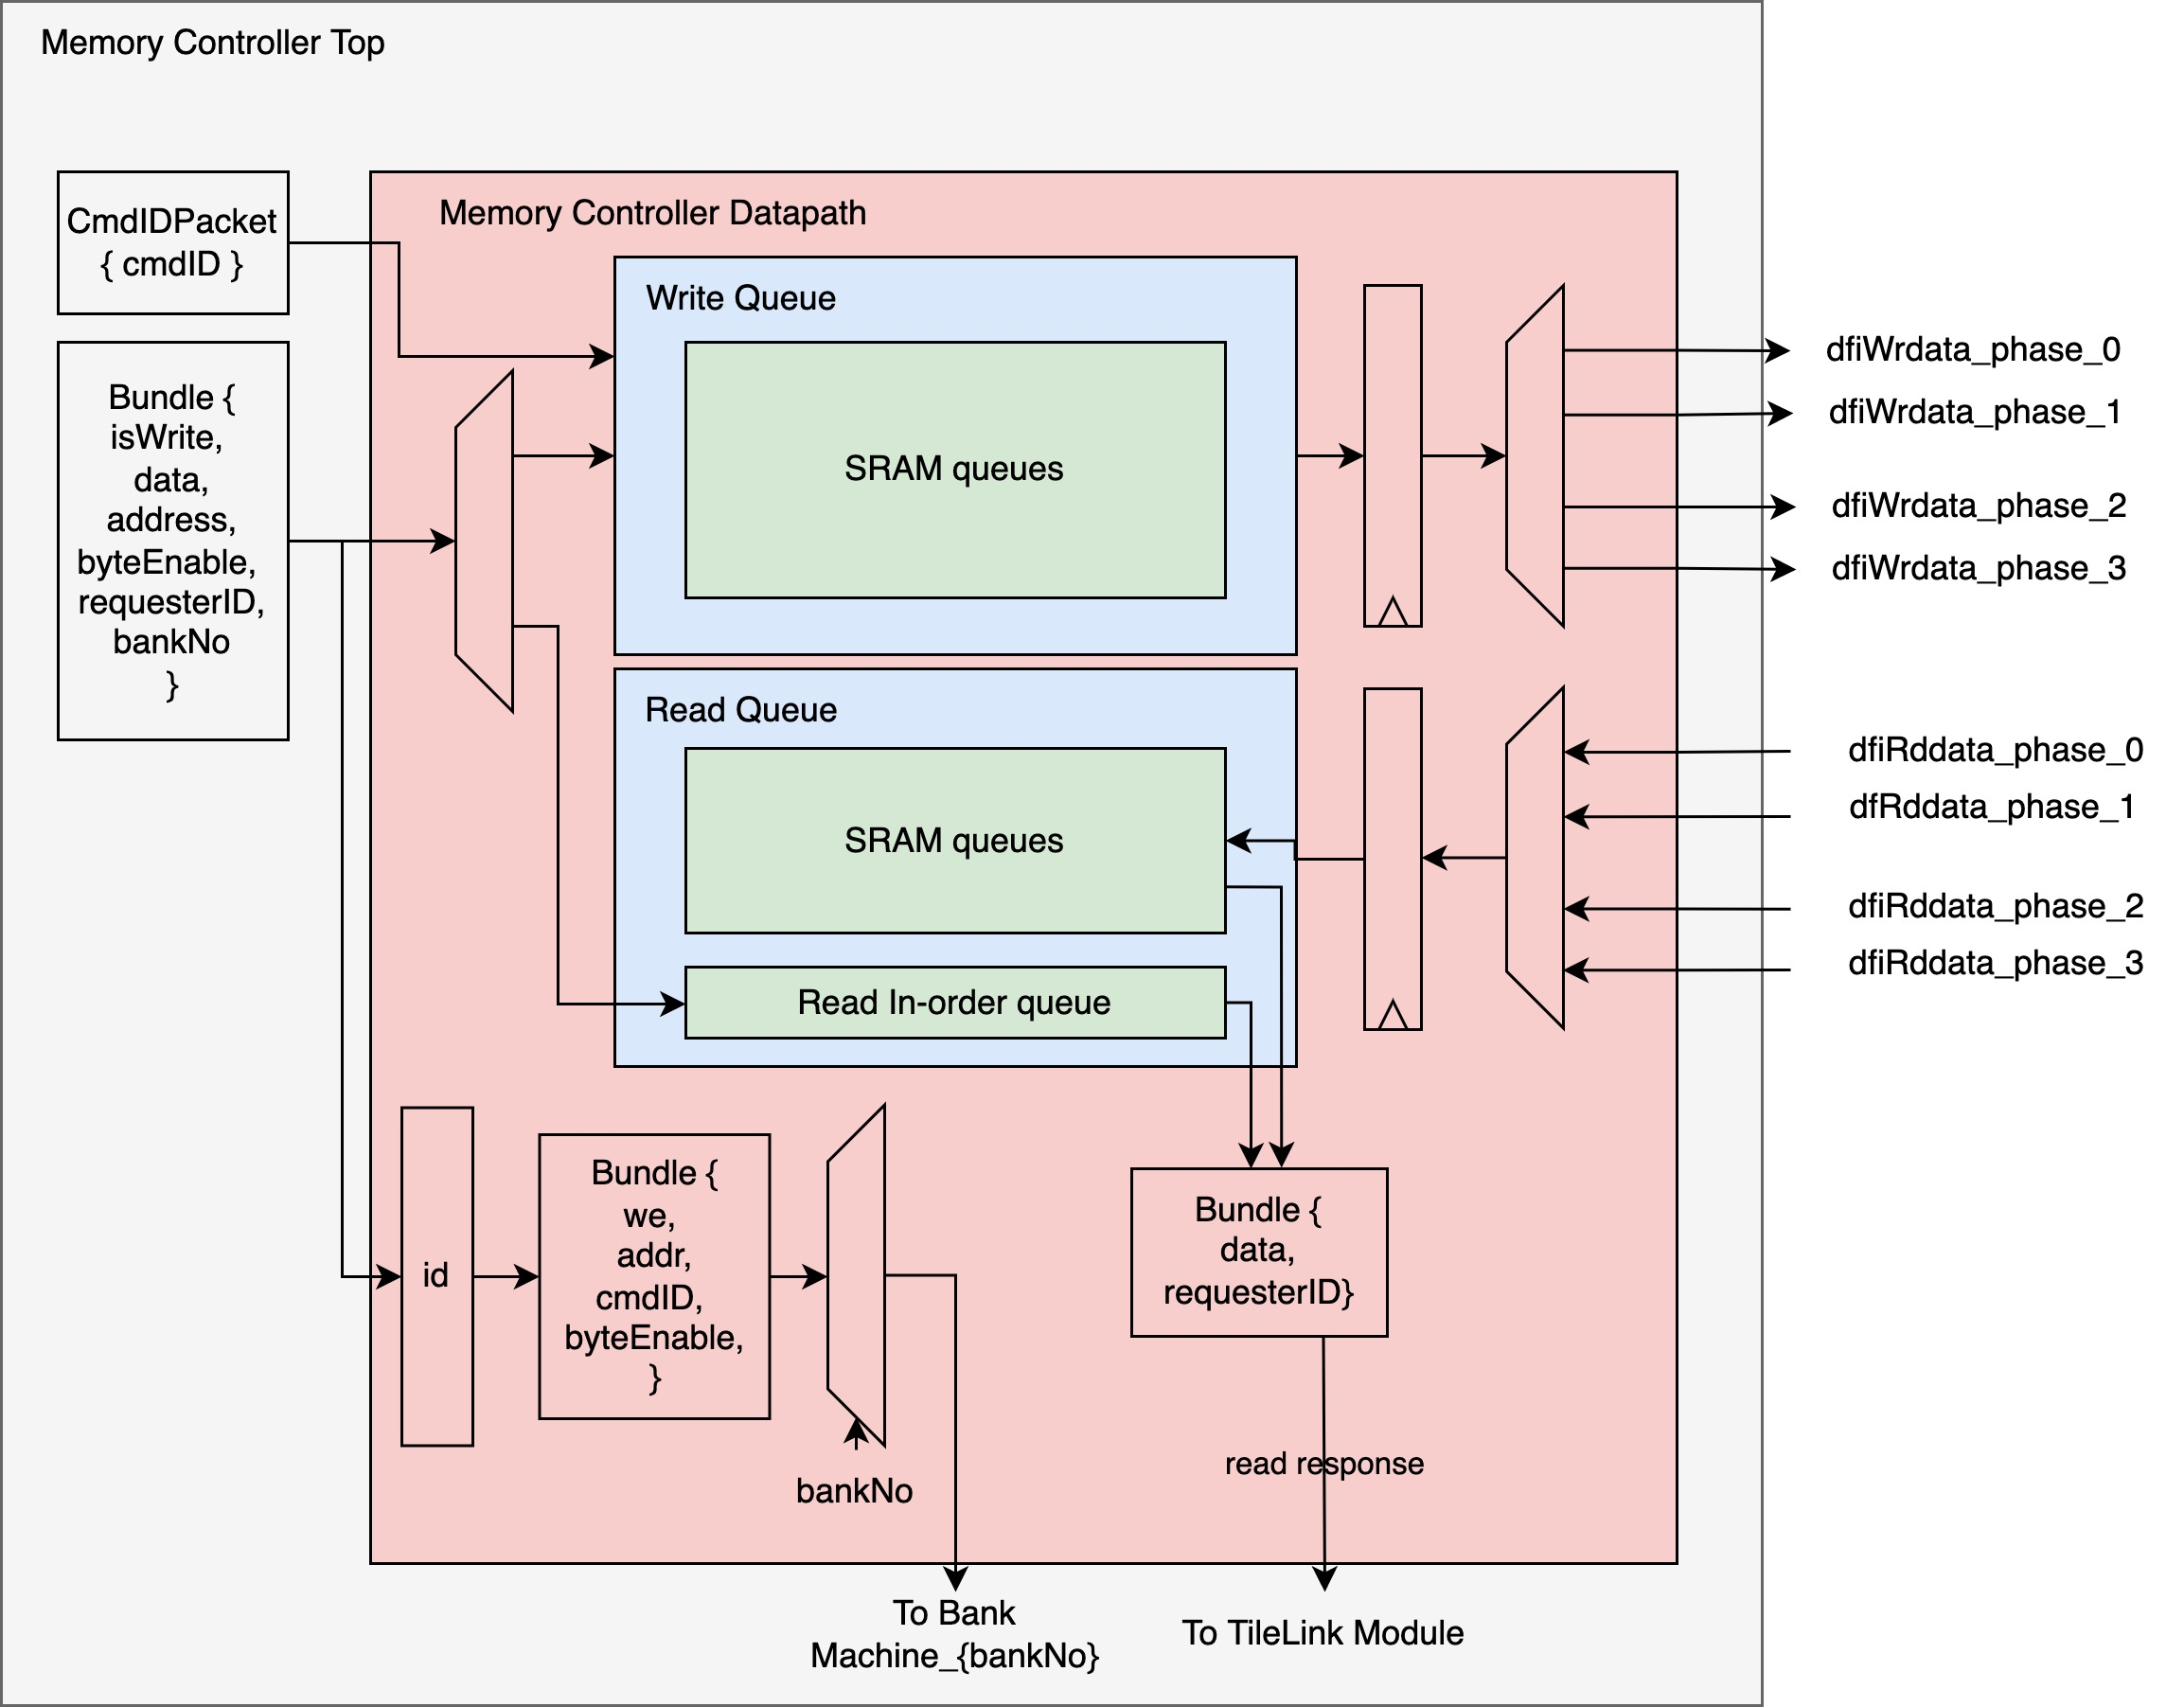
\includegraphics[scale=0.2]{images/datapath-u.jpg}
    \caption{Datapath internal logic.}
    \label{fig:data_uarch}
\end{figure}
\begin{figure}
    \centering
    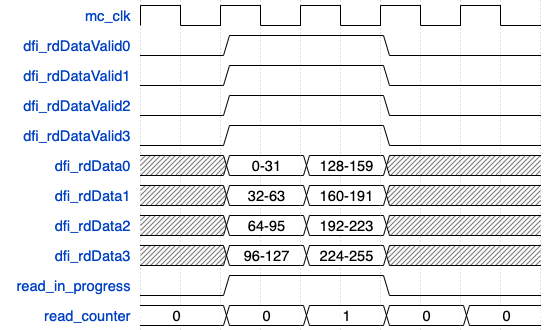
\includegraphics[scale=0.5]{images/read-capture.png}
    \caption{Capturing of DFI read response.}
    \label{fig:read-cap}
\end{figure}
\begin{figure}
    \centering
    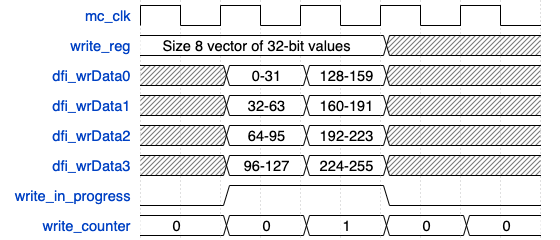
\includegraphics[scale=0.5]{images/writes-to-dfi-mod.png}
    \caption{Transmission of DFI write data.}
    \label{fig:write-trans}
\end{figure}
\newpage
\section{TileLink Lazy Module}
TileLink elaboration depends on a lazy system to connect the nodes together and avoid a deadlock in the bus system. A TileLink node would be instantiated in the system at the time of elaboration. In case there are mismatches between the bus width, the TileLink diplomacy monitors' assertions would stop the compilation process. The deadlock-free requirements are also checked at the compile time. Our design relies on API provided by Diplomacy to create a manager node as well as a register node in the TileLink lazy module.

The manager node connects to the Memory Bus of the system and accepts packets on channel A of TileLink. We have designed our manager node to be compatible with the TL-UL protocol. TL-UL is a TileLink Uncached Lightweight protocol that requires channel A and D implementations. Data in the DRAM is not cached and as a result, the TileLink node for the memory controller does not need to implement channels B and C. The controller manager node for the controller can only accept packets that are one beat only. In large SoC with wider bus widths, TileLink adopts a multi-beat packet protocol. In such systems, a \verb|Fragmenter| module is instantiated automatically to translate the multi-beat packets to one packet and vice versa. The \verb|Fragmenter| takes in as input a multi-beat packet and once the packet is fully transmitted, sends the constructed one-beat packet to the controller. It can also perform the same logic in the opposite direction where the controller can produce a one-beat packet and send it to the \verb|Fragmenter|, which internally breaks up the packet into a multi-beat packet.

\section{Synthesis Result}
We synthesized the design as part of our initial assessment phase of the tape-out process using Hammer, a physical design flow tool \cite{10.1145/3489517.3530672}. The reports are based on Intel 16 technology which is a 22 nm FinFET process node. The synthesis report indicates a relatively small area footprint. The synthesis report in table \ref{tab:syn_report} shows the instance types used from the technology library.

In table \ref{tab:area}, the subsequent area report shows a breakdown of our memory controller by modules. Note that all area units are in micro-meter squared.
\begin{table}[H]
    \centering
    \begin{tabular}{c|c|c|c}
         Type & Instances & Area & \% Area  \\
         \hline
         Sequential & 6973 & 9529 & 64.9 \\
         Inverter & 897 & 183 & 1.2 \\
         Buffer & 39 & 35.109 & 0.2 \\
         Clock Gate & 420 & 657 & 4.5 \\
         logic & 10022 & 4284  & 29.2 \\
         total & 18351 & 14690 & 100.0 \\
    \end{tabular}
    \caption{Synthesis report.}
    \label{tab:syn_report}
\end{table}

\begin{table}[H]
    \centering
    \begin{tabular}{c|c|c|c}
    Instance & Module & Cell Count & Total Area \\
    \hline
    top & MemoryControllerTop & 18351 & 18961.802 \\
    core & MemoryControllerCore & 8759 & 8371.554 \\ 
    datapath & MemoryControllerDataPath & 9128 & 10099.057\\
    \end{tabular}
    \caption{Area breakdown by module.}
    \label{tab:area}
\end{table}
\chapter{Software Model}
To perform design space exploration, a software model written C++ language is provided with the generator. The generator can be then exercised with this software model without performing costlier and longer RTL simulations. In addition, a software model can be used to find bottlenecks in the system and optimize the RTL based on the findings. Parameterization of the RTL modules in a software model is much more intuitive which allows for fast iterations on multiple parameters for a specific design without elaborating the SoC and controller RTL. 
\section{Cycle Information}
It is important to model the controller with clock and cycle information so that a possible bottleneck in the system can be found. In the software model, we added a \verb|Clock| class to model the system using an object of the \verb|Clock|. A \verb|Clock| object provides the API necessary to set the clock to a certain cycle, and tick the clock. The \verb|Clock| API is shown below.
\begin{verbatim}
class Clock {
private:
  std::string clock_name;
  uint64_t cycle;
public:
  Clock(std::string name);
  void set_to_cycle(uint64_t cc);
  uint64_t get_cycle();
  void tick();
};
\end{verbatim}
Using clock objects allows us to output the progress of transactions with the cycle information.
\section{Issuers}
A \verb|TransactionIssuer| is used to model software running on the system. Since the software model does not exactly need to adhere to the specific hardware protocols, we can avoid detailed signals within a TileLink packet and summarize a transaction as below:

\begin{verbatim}
enum TXType {
  read, 
  write
};

typedef struct Transaction {
  uint64_t id;
  uint64_t address;
  uint32_t sourceId;
  uint8_t bank;
  TXType opcode;
  std::vector<uint64_t> data;
  uint64_t mask;
} Transaction;
\end{verbatim}
A \verb|TransactionIssuer| is a c++ class that can read transactions from a provided transaction stream in a text format. The object can also generate random transactions and issue them to the controller.
The \verb|TransactionIssuer| interface is as shown below:
\begin{verbatim}
class TransactionIssuer {
private:
  std::string name;
  uint16_t sourceId;
  std::map<uint64_t, Transaction*> awaiting;
  std::map<uint64_t, Transaction*> processed;
public:
  TransactionIssuer(std::string this_name, uint16_t sid);
  std::string get_name();
  uint16_t get_source_id();
  std::map<uint64_t, Transaction*> get_awaiting_tx();
  Transaction* get_random_tx(uint64_t cycle);
  void read_tx_from_file(std::string f);
\end{verbatim}
The awaiting and processed fields can be used to monitor the progress of the controller on issuing the transactions and the responses from the DRAM software model. 
\section{Dram Memory Model}
A simple memory model would suffice for this software model as the purpose of this model is to realize the functionality and performance of the memory controller. Therefore, a zero-latency model for memory transactions can be used. A simple mapping of addresses to 256-bit values with an additional map to keep track of the state of each row is used for modeling a bank in the DRAM device. The \verb|Bank| class is defined with core functionalities and zero latencies for all the commands: 
\begin{verbatim}

class Bank {
private:
  State state;
  uint64_t active_row;
  uint8_t bank;
  std::map<uint64_t, DramData*> mem;
public: 
  Bank(uint8_t i) {
    bank = i;
    state = IDLE;
  }
  void activate(uint64_t addr);
  void precharge();
  void refresh();
  DramData* read_cas(uint64_t addr, bool auto_pre);
  void write_cas(uint64_t addr, DramData *data, bool auto_pre);
};
\end{verbatim}
A full DRAM model uses the Bank class and instantiates eight banks. It then exposes the same methods and dispatches the calls to the corresponding bank based on the address. As an example, the activate method in the \verb|DramModel| extracts the bank bits from the address and then dispatchers the \verb|activate| call to the corresponding bank.
\begin{verbatim}
class DramModel {
private:
  uint64_t capacity;
  Bank *banks[8];
  uint8_t get_bank_from_addr(uint64_t addr) {
    return (uint8_t)(addr & (7 << 9));
  }
  uint64_t no_bank_bits(uint64_t addr);
public:
  DramModel(uint64_t cap);
  void activate(uint64_t addr) {
    uint8_t bn = get_bank_from_addr(addr);
    banks[bn]->activate(no_bank_bits(addr));
  }
  void precharge_all_banks();
  void precharge(uint64_t addr);
  void refresh_all_banks();
  DramData* read_cas(uint64_t addr, bool auto_pre);
  void write_cas(uint64_t addr, DramData *data, bool auto_pre);
};
\end{verbatim}
The above API can perform the main commands of the DRAM. We avoided the implementation of complete JEDEC accurate commands since this model is not used for verification purposes of the controller.
\section{Core Model}
The Core model consists of the wrapper class around the eight Bank Machine classes with a command chooser and the multiplexer. A cycle per cycle function calls to the \verb|fsm| function of each Bank Machine object would trigger them to process a command and return a possible command if the timing parameters are met. The timing parameters are implemented as variables that are modified by the \verb|fsm| function. On each cycle, if there exists a command that meets the timings and can be issued, the \verb|fsm| method of the Bank Machine returns the corresponding Bank Output structure. The structures implemented in the software model have the same fields as the bundles in our RTL. 

A command selection logic uses a round-robin implementation in software and picks between one of the possible eight outputs from the \verb|fsm| method of each Bank Machine. The output of the Core object then is multiplexed with the other controllers such as the refresh controller and then sent out to the DRAM memory model.

\chapter{Conclusion}
\section{Summary}
During the course of this program, I worked on the implementation, architectural design, and verification of an LPDDR4X memory controller. 

Our goal was to create a generator that can be integrated into Chipyard and used in future chip designs and research. 

During our development phase, we tested the functionality of units and verified our logic. In addition, we have a simulation-based test harness where we exercise the end-to-end system as a whole. 

\

\section{Future Work}
Optimizations of the architecture and micro-architecture of the controller, formal verification, and a more robust test harness are some of the future work for this project. I will keep contributing to the project whenever possible and will mainly focus on a complete software model for this design.

The implementation will be taped-out in the near future and will be brought up as a design under a test environment for the purpose of post-silicon validation. We completed our mission of a complete generator for LPDDR4X. However, there will be extended research on optimizing the controller architecture, PHY design, and PCB design mainly by Ken Ho and other graduate students. 

\printbibliography
\end{document}
